\documentclass[twoside, 12pt]{report}

% --- PACCHETTI ---

% unità di misura
\usepackage{siunitx}

% titolo capitoli e sezioni personalizzato
\usepackage{titlesec}

\titleformat{\chapter}
{\normalfont\LARGE\bfseries}{\thechapter.}{10pt}{\LARGE}
\titlespacing*{\chapter}{0pt}{0pt}{20pt}

\titleformat{\section}
{\normalfont\large\bfseries}{\thesection}{10pt}{\large}
\titlespacing*{\section}{0pt}{0pt}{10pt}

% include pdfs
\usepackage{pdfpages}

% grafiche e tabelle
\usepackage{graphicx}
\usepackage{calc}

\graphicspath{{images/}}

\usepackage{tikz}
\usepackage{pgfplots}
\usepackage{pgfplotstable}

\pgfplotsset{compat = newest}
\usepgfplotslibrary{units}

\pgfplotstableset{% global config
    col sep = comma,
    string type,
    every last row/.style = {after row = \hline},
    every even row/.style = {
        before row = \hline\rowcolor{myLightBlue},
        after row = \hline,
    },
}

% colori personalizzati
\usepackage{colortbl}
\usepackage{xcolor}

% normali
\definecolor{myBlue}{RGB}{1, 187, 235}
\definecolor{myRed}{RGB}{255, 43, 43}
\definecolor{myYellow}{RGB}{255, 221, 86}
\definecolor{myBlack}{RGB}{28, 28, 28}
\definecolor{myGrey}{RGB}{134, 134, 134}
% chiari
\definecolor{myLightBlue}{RGB}{177, 239, 255}
\definecolor{myLightRed}{RGB}{255, 177, 177}
\definecolor{myLightYellow}{RGB}{255, 240, 180}
\definecolor{myLightGrey}{RGB}{218, 218, 218}

\pgfplotscreateplotcyclelist{modular}{
        {myBlue},
        {myRed},
        {myYellow},
        {myBlack},
        {myGray},
      }

\usepackage{subcaption}

\usepackage{csvsimple}

% numerazione capitoli in italiano
\usepackage[italian]{babel}

% spaziatura
\usepackage{parskip}

% impaginazione
\usepackage{setspace} % For doublespacing

\doublespacing

\usepackage{geometry}

\geometry{a4paper, top = 2cm, bottom = 2cm, outer = 2cm, inner = 3cm, heightrounded}

% font
\usepackage{times}

% bibliografia
\usepackage{csquotes}
\usepackage{biblatex}

\addbibresource{bibliography.bib}

\usepackage{xurl} % evita che la bibliografia esca dal margine
\usepackage{url}

\urlstyle{same}
\appto{\bibsetup}{\raggedright}

% salta pagine bianche
\usepackage{afterpage}

\newcommand\emptypage{
    \newpage
    \thispagestyle{empty}
    \mbox{}
    \newpage
}

% riempimento testo dummy per prova
\usepackage{lipsum}

% interlinea
\linespread{1.5}

% comandi per aggiungere chapter, section e subsection non numerate al toc
\newcommand\unchapter[1]{
    \chapter*{#1}
    \addcontentsline{toc}{chapter}{#1}}

\newcommand\unsection[1]{
    \section*{#1}
    \addcontentsline{toc}{section}{#1}}

\newcommand\unsubsection[1]{
        \subsection*{#1}
        \addcontentsline{toc}{subsection}{#1}}

% --- DOCUMENTO PRINCIPALE ---

% inizio del documento
\begin{document}

% --- FRONTESPIZIO ---
% DA MODIFICARE DATA DI LAUREA !!!

\includepdf{pdfs/frontespizio/frontespizio_tesi.pdf}
\emptypage

% --- INDICE ---

\tableofcontents
\emptypage

% --- CAPITOLI ---

\unchapter{Introduzione e Specifiche di Progetto}

%--------------------------------------------------------------------------------------------

In questa tesi viene discussa la progettazione di un sintetizzatore musicale compatibile con
lo standard modulare più diffuso al giorno d'oggi, ovvero Eurorack \cite{eurorack}. Più
precisamente si vuole realizzare un generatore di segnali che offra la possibilità di essere
controllato in tensione (Voltage Controlled Oscillator, o VCO in breve). In questo modo,
applicando dei segnali variabili nel tempo in ingresso al modulo, si è in grado di variare
dinamicamente la frequenza dei segnali in uscita.

Il range scelto per tale variazione comprende la fascia di frequenze utili nello spettro
audio, quindi da poche decine di $Hz$ a circa $7kHz$. Si desidera inoltre, la possibilità di
convertire a piacere il funzionamento del modulo in oscillatore a bassa frequenza (Low Frequency
Oscillator, o LFO), spostando quindi il range di frequenze disponibili da frazioni di
$Hz$ a qualche decina di $Hz$.
\medskip

\begin{figure}[ht]
    \centering
    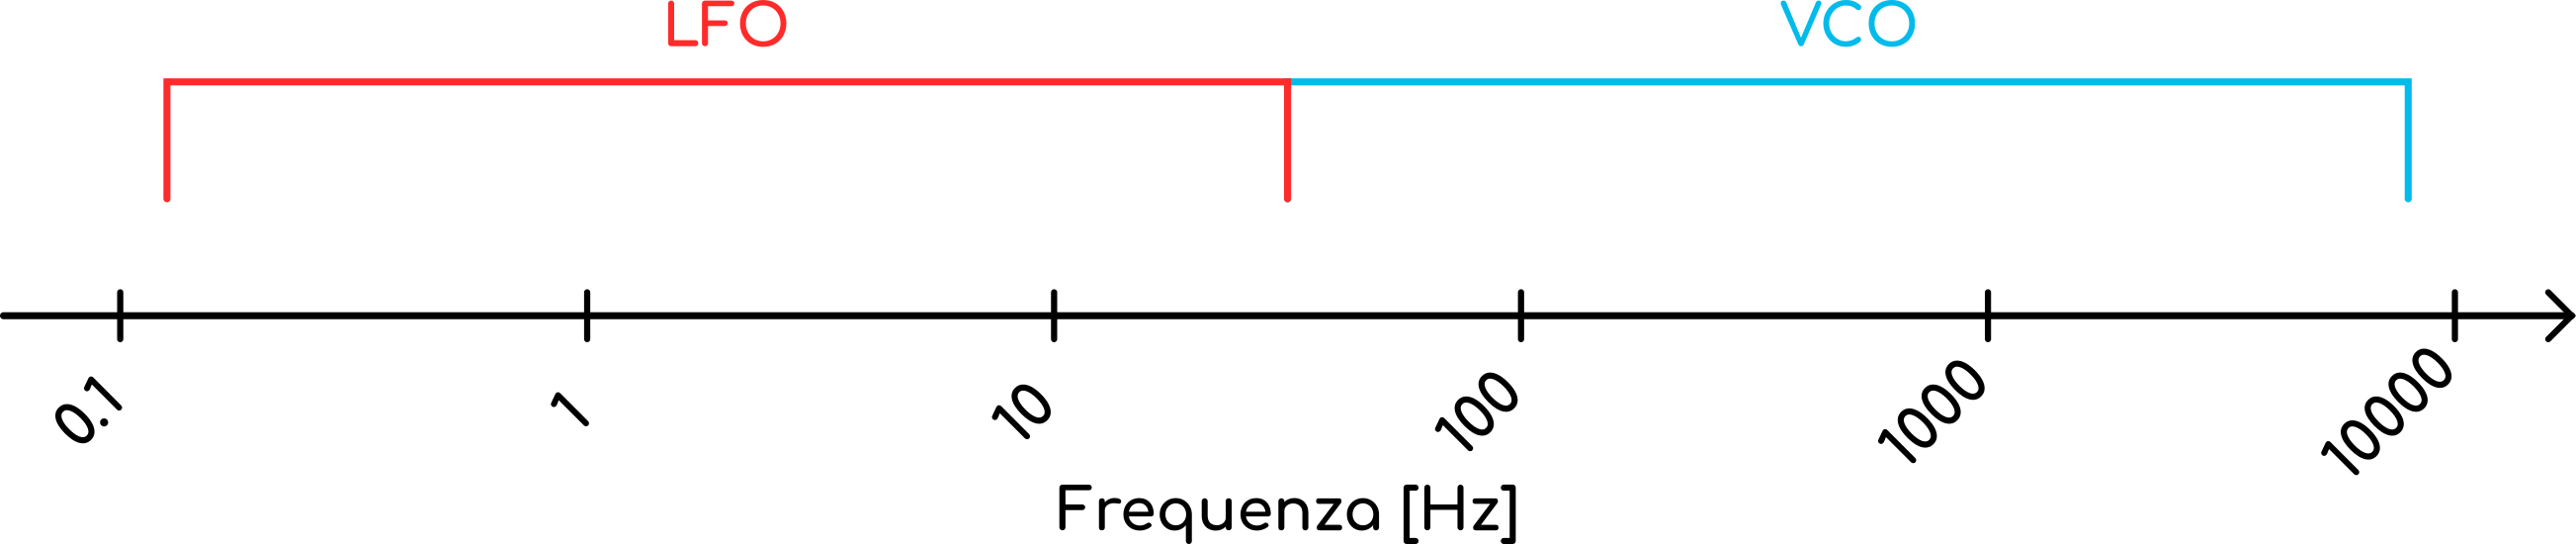
\includegraphics{graphs/functioning_range.png}
    \caption{Range di funzionamento in scala logaritmica}
    \label{functioning_range}
\end{figure}

In modalità VCO quindi, il modulo produrrà dei segnali che attraverso un adeguato sistema
potranno essere ascoltati, mentre in modalità LFO il circuito produrrà dei segnali lentamente
variabili nel tempo, utili per la modulazione e il controllo di parametri in altri moduli
eventualmente presenti nel sistema.

Le forme d'onda desiderate sono quelle base, ovvero:

\begin{itemize}
    \item Sinusoide;
    \item Onda Quadra;
    \item Triangolo;
    \item Rampa;
    \item Dente di sega (sebbene nel range VCO non risulti particolarmente differente dalla
          rampa in termini di suono, per quanto riguarda il funzionamento LFO la differenza
          è radicale, poichè il segnale viene solitamente utilizzato come modulante);
\end{itemize}

inoltre, come verrà illustrato più avanti, risulta piuttosto semplice anche estrarre un
segnale a impulso, rigorosamente alla stessa frequenza di quelli già generati. Tale segnale
può essere utilizzato per scopi simili a quelli dei segnali in uscita in modalità LFO.
\smallskip

Per quanto riguarda le specifiche sui livelli di tensione, si vogliono imporre i seguenti
intervalli di valori:

\begin{itemize}
    \item Segnali audio (i 5 elencati poco sopra): $\pm5V$;
    \item Segnali logici (impulso): $(0V,5V)$;
    \item Tensione di ingresso: $(0V,8V)$ in modalità $1V/Octave$, ovvero facendo in modo che
          ad un incremento di $1V$ corrisponda un raddoppio di frequenza, cioè un'ottava;
    \item Alimentazioni: $\pm12V$ e $+5V$;
\end{itemize}

Le specifiche sopra riportate sono prese dallo standard Eurorack.

Altre caratteristiche volute sono:

\begin{itemize}
    \item Manopole per il controllo del "volume" di segnali in ingresso e uscita, ad eccezione
          dell'impulso;
    \item Manopole per il controllo manuale della frequenza;
\end{itemize}

Raccogliendo tutti questi dettagli possiamo iniziare a pensare ad una interfaccia utente,
riportata in figura \ref{panel_explained}, in modo da rendere più chiaro al lettore il
prodotto finale.
\medskip

\begin{figure}[ht]
    \centering
    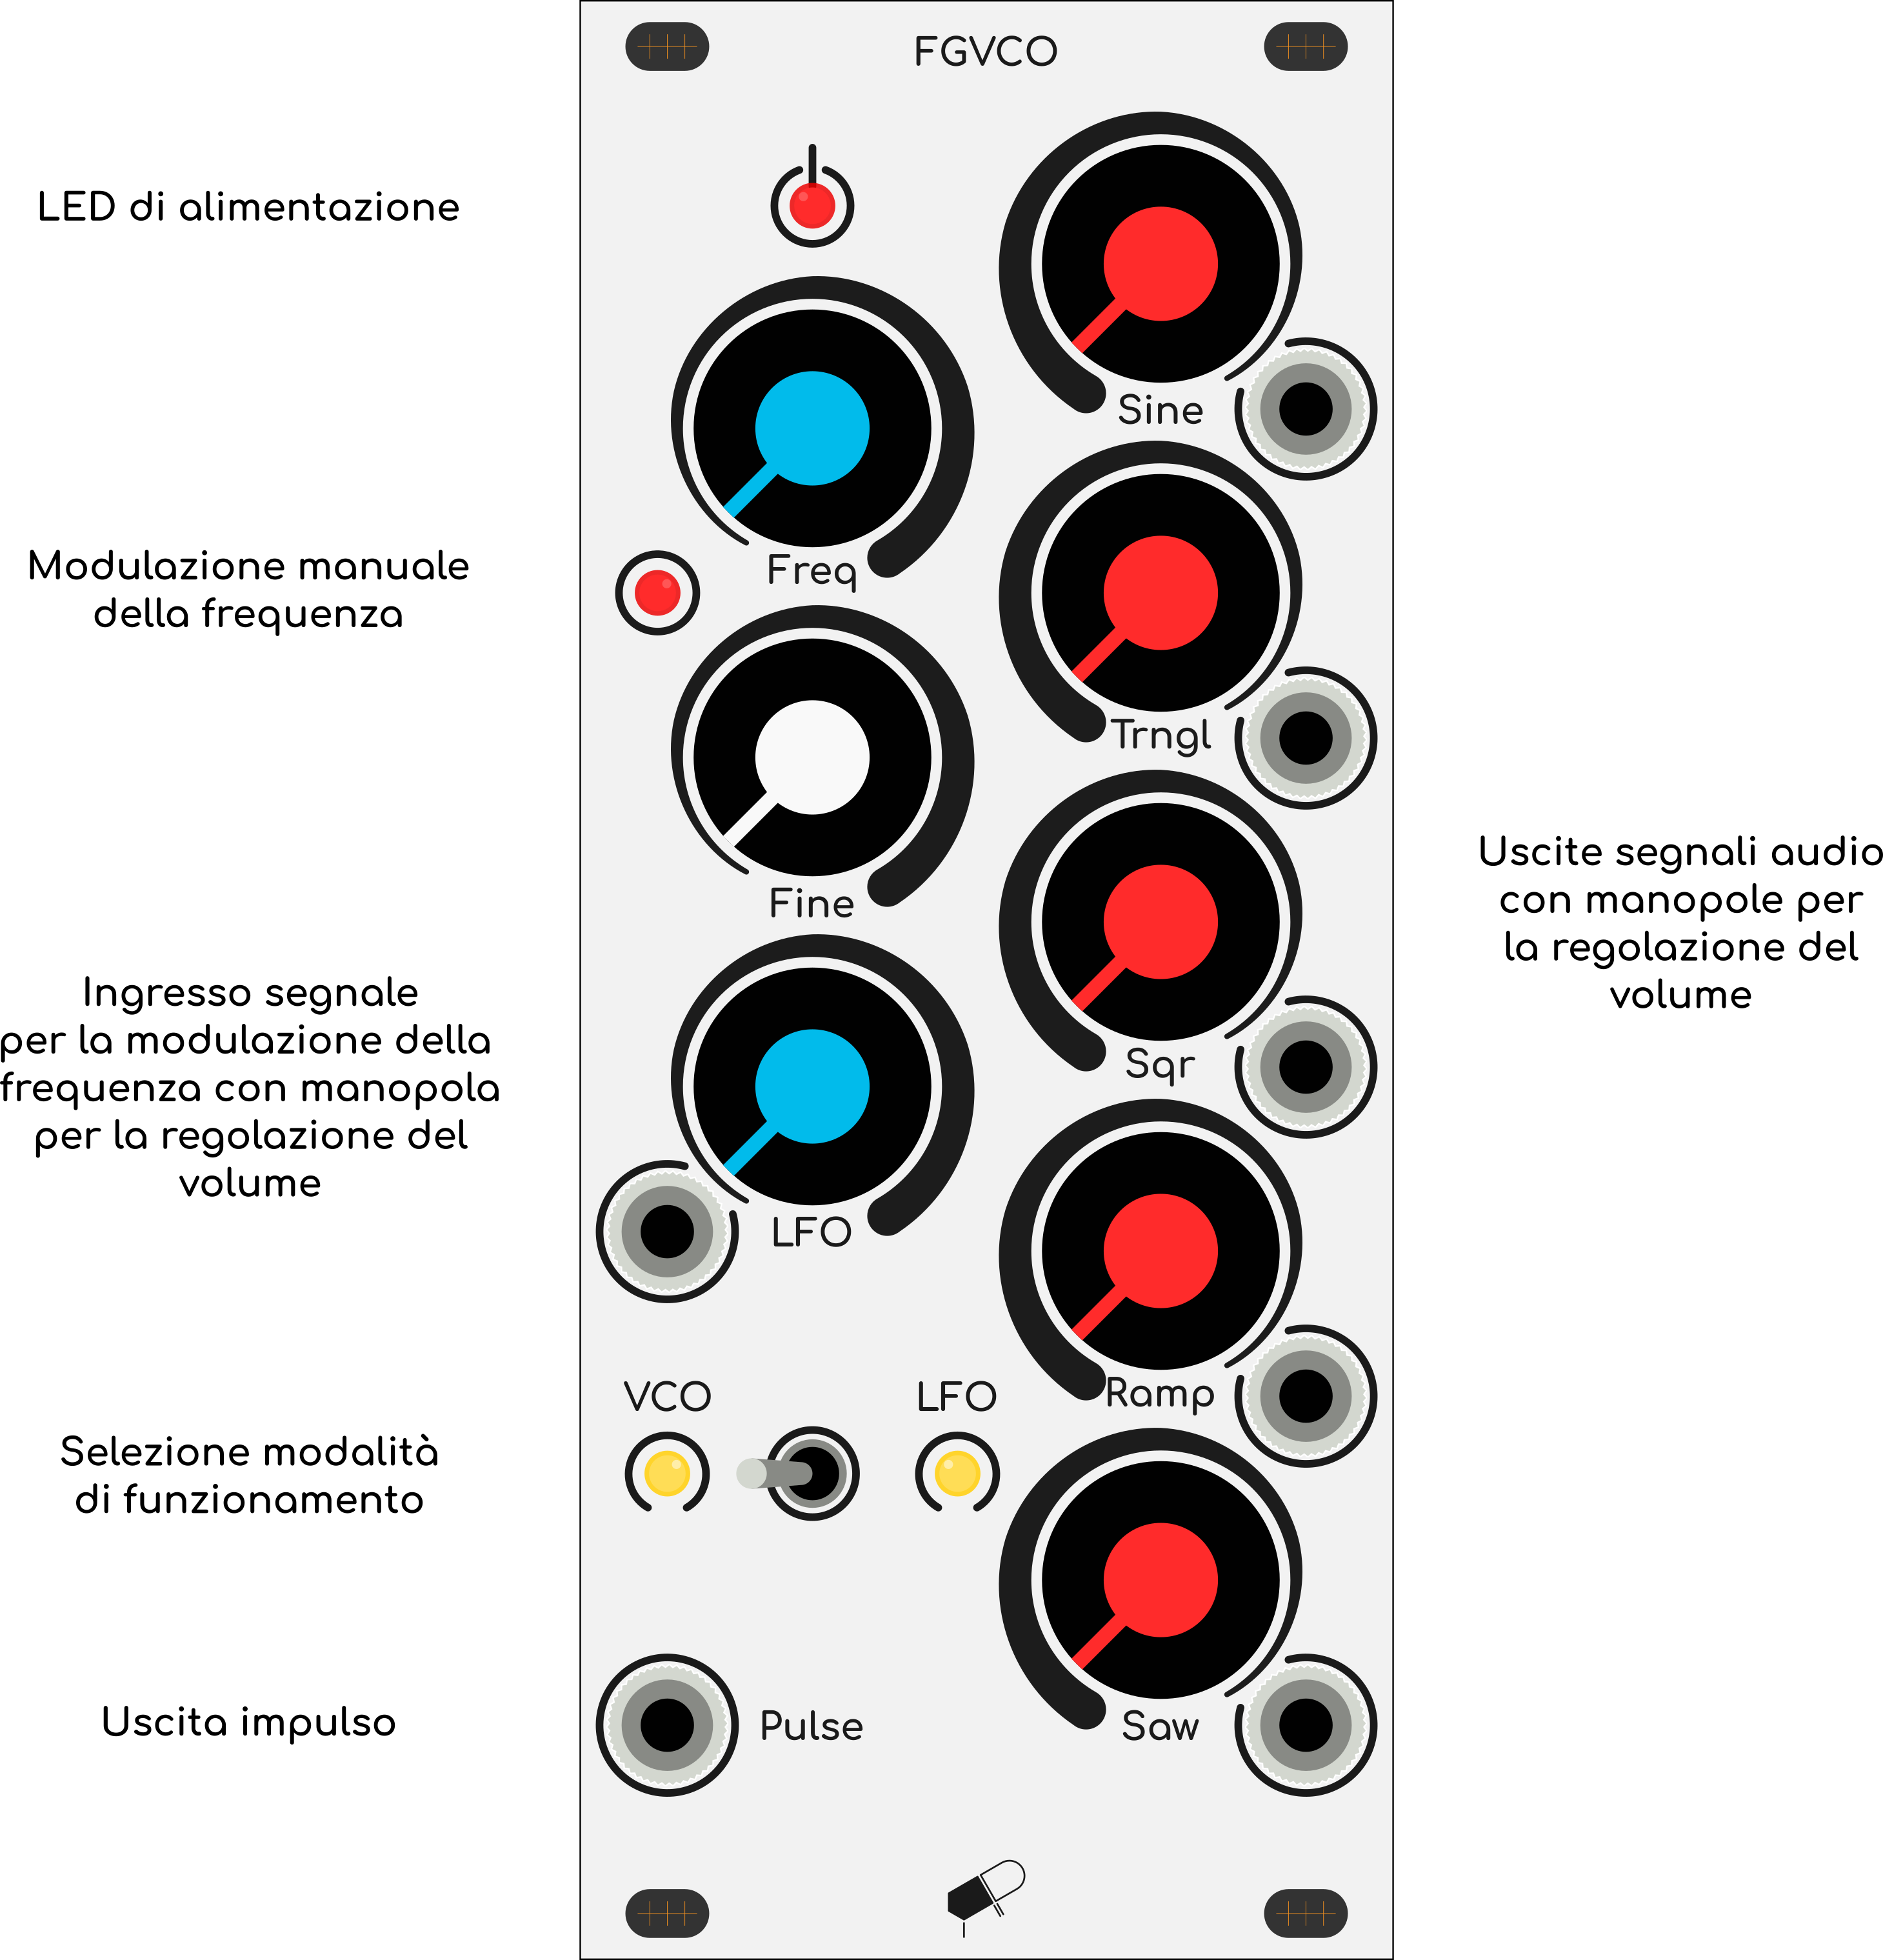
\includegraphics{misc/panel_explained.png}
    \caption{Pannello frontale del modulo}
    \label{panel_explained}
\end{figure}

Si decide di realizzare l'intero circuito senza l'utilizzo di microcontrollori o sistemi
programmabili. Tale scelta viene presa per mettere alla prova più competenze possibili tra
quelle acquisite durante gli anni di studio. Si potrebbe infatti realizzare il tutto con un
microcontrollore dotato di forme d'onda densamente campionate salvate in memoria.
Altro motivo per il quale si sceglie questa strada è per avere ogni segnale su un canale
a sè in modo da poter usufruire di ognuno contemporaneamente.

%--------------------------------------------------------------------------------------------

\chapter{Generazione dei Segnali Principali}

%--------------------------------------------------------------------------------------------

Per la generazione dei segnali a rampa e a triangolo si decide di procedere in ogni caso
per via digitale, utilizzando dei contatori binari abbinati ad un convertitore
digitale-analogico.
\medskip

\begin{figure}[ht]
    \centering
    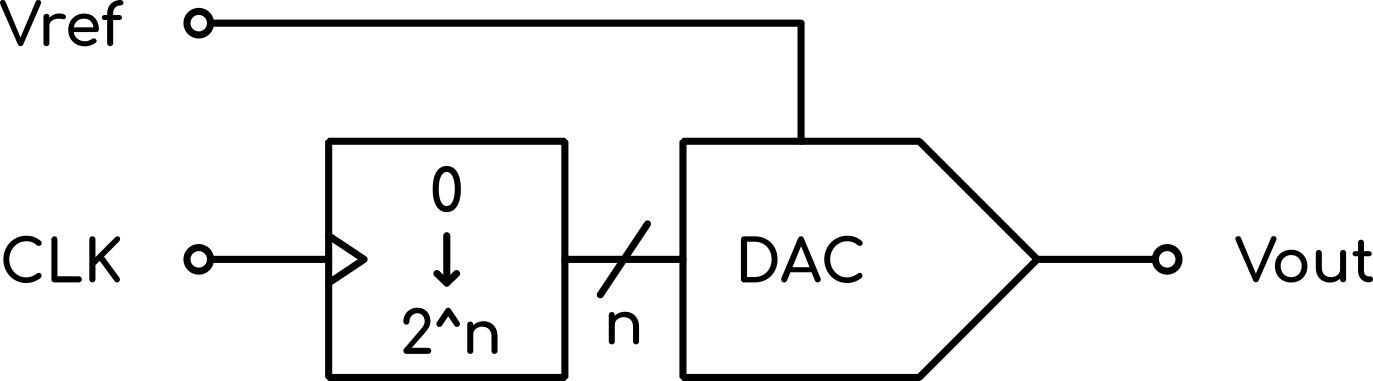
\includegraphics{block_diagrams/counter_block_diagram.png}
    \caption{Schema a blocchi generale di un generatore di segnale}
    \label{counter_block_diagram}
\end{figure}

%--------------------------------------------------------------------------------------------

\section{Rampa}

%--------------------------------------------------------------------------------------------

\subsection*{Principio di Funzionamento}

%--------------------------------------------------------------------------------------------

Per il segnale a rampa si fa uso di un contatore unidirezionale, ovvero un dispositivo
in grado di contare automaticamente da $0$ a $2^n$, dove $n$ corrisponde al numero di bit,
semplicemente fornendo un segnale di clock adeguatamente dimensionato. Maggiore il numero
di bit $n$, maggiore sarà la precisione del nostro segnale, quindi minore l'intensità del
rumore generato.
\medskip

\begin{figure}[ht]
    \centering

    \begin{subfigure}{.5\textwidth}
        \centering
        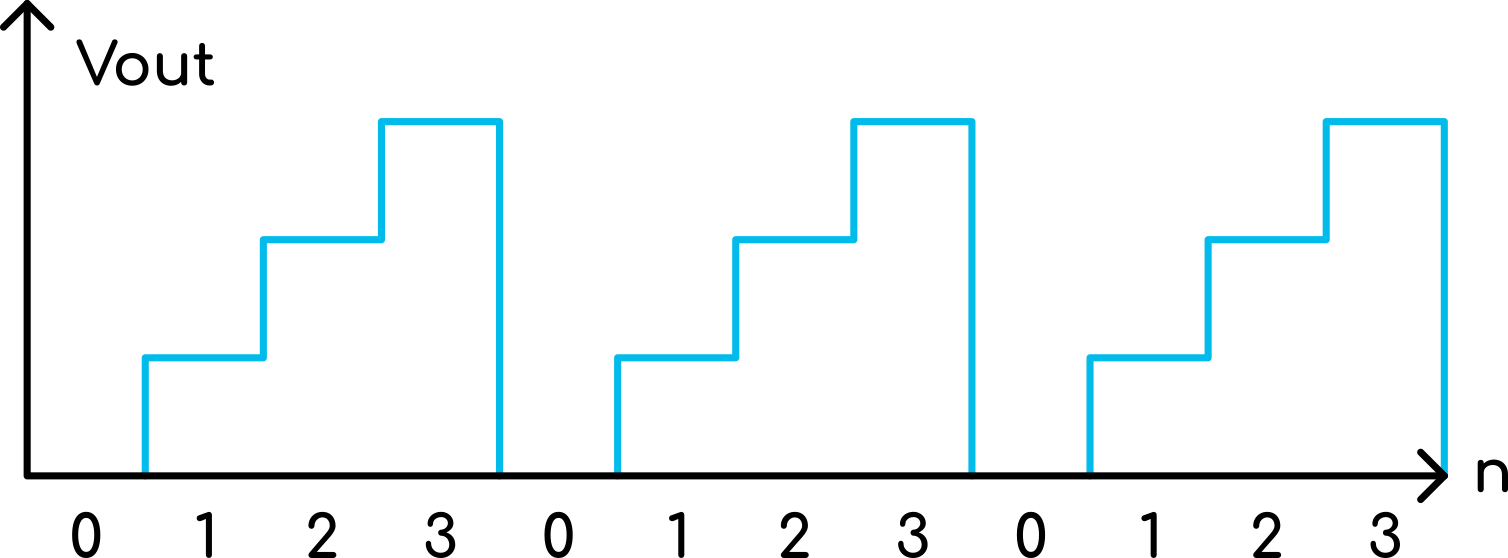
\includegraphics{graphs/low_res_ramp.png}
        \caption{Rampa ottenuta con un contatore a 2 bit}
        \label{low_res_ramp}
    \end{subfigure}%
    \begin{subfigure}{.5\textwidth}
        \centering
        
\includegraphics{graphs/high_res_ramp.png}
        \caption{Rampa ottenuta con un contatore a 8 bit}
        \label{high_res_ramp}
    \end{subfigure}

    \caption{Confronto tra contatori unidirezionali con diverso numero di bit}
    \label{ramps}
\end{figure}

Tuttavia aumentando il numero di bit del contatore è facile intuire che, a parità di
frequenza del segnale in uscita, la frequenza del segnale di clock debba necessariamente
aumentare.

Vale infatti la seguente relazione:

\begin{displaymath}
    f_{signal}=\frac{f_{clk}}{2^n}[Hz]
\end{displaymath}

poichè il contatore deve effettuare un conteggio completo durante un periodo del segnale
in uscita. Questo implica dunque un limite massimo al numero di bit del contatore.

La quantità di bit utilizzati per l'applicazione è $8$, valore che ci consente di limitare
al $MHz$ la frequenza di clock, contare fino a $255$ e dividere l'intervallo di tensione
d'uscita in altrettanti livelli, ottenendo quindi una variazione di

\begin{displaymath}
    V_{step}=\frac{2V_{ref}}{2^n}=\frac{10V}{256}\approx39mV
\end{displaymath}


per ogni singolo bit (scegliendo $V_{ref}=+5V$).
\medskip

\begin{figure}[ht]
    \centering
    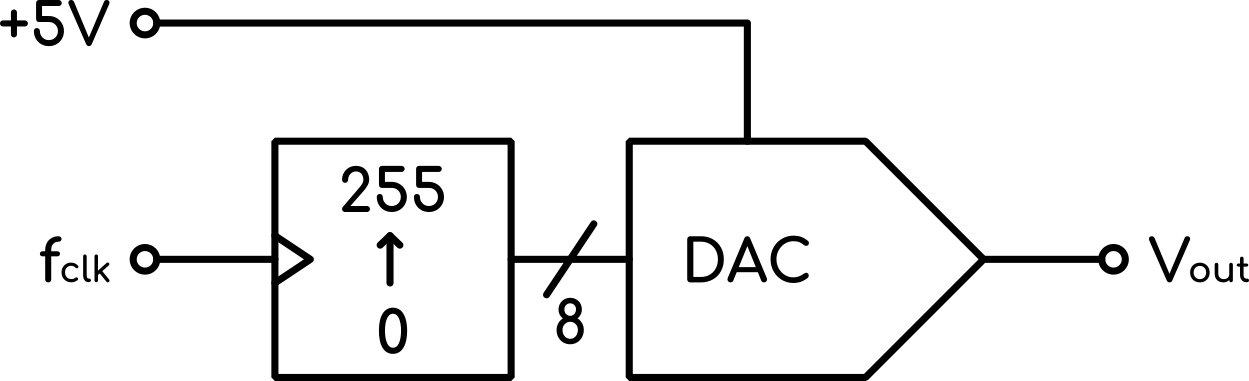
\includegraphics{block_diagrams/ramp_block_diagram.png}
    \caption{Schema a blocchi del sottosistema per la generazione della rampa}
    \label{ramp_block_diagram}
\end{figure}

A questo punto possiamo calcolare le speccifiche del segnale di clock da generare,
andando a vedere quali sono le frequenze desiderate per i segnali audio:

\begin{itemize}
    \item Valore minimo (nota A0): $f_{signal-min}=27.5Hz\rightarrow f_{clk-min}\approx7kHz$
          a cui corrisponderà un ingresso di $0V$;
    \item Valore massimo (nota A8): $f_{signal-max}\approx7kHz\rightarrow f_{clk-max}\approx1.8MHz$
          a cui corrisponderà un ingresso di $8V$;
\end{itemize}

ovvero un range di funzionamento esteso lungo 8 ottave.

%--------------------------------------------------------------------------------------------

\subsection*{Componenti Utilizzati e Schemi Elettrici}

%--------------------------------------------------------------------------------------------

Si passa ora alla scelta dei componenti per la realizzazione del blocco circuitale.

\begin{itemize}
    \item Contatore: 74HC590 \cite{74hc590};
    \item DAC: DAC0800 \cite{dac0800};
\end{itemize}

Per il circuito DAC si utilizza lo schema a pg.10 del relativo datasheet del componente.
Tale configurazione ci permette infatti di convertire il dato binario in un valore compreso
nell'intervallo $\pm V_{ref}= \pm 5V$, tuttavia si utilizzano un amplificatore
operazionale e dei resistori di valore differente (rispettivamente TL074 \cite{tl074} e
$R_L=\bar{R_L}=3.3k\Omega$). Si noti che anche $V_{ref}$ viene scelta diversa rispetto allo
schema nel datasheet ($+5V$), in modo da garantire le specifiche di progetto sul segnale
in uscita.
\medskip

\begin{figure}[ht]
    \centering
    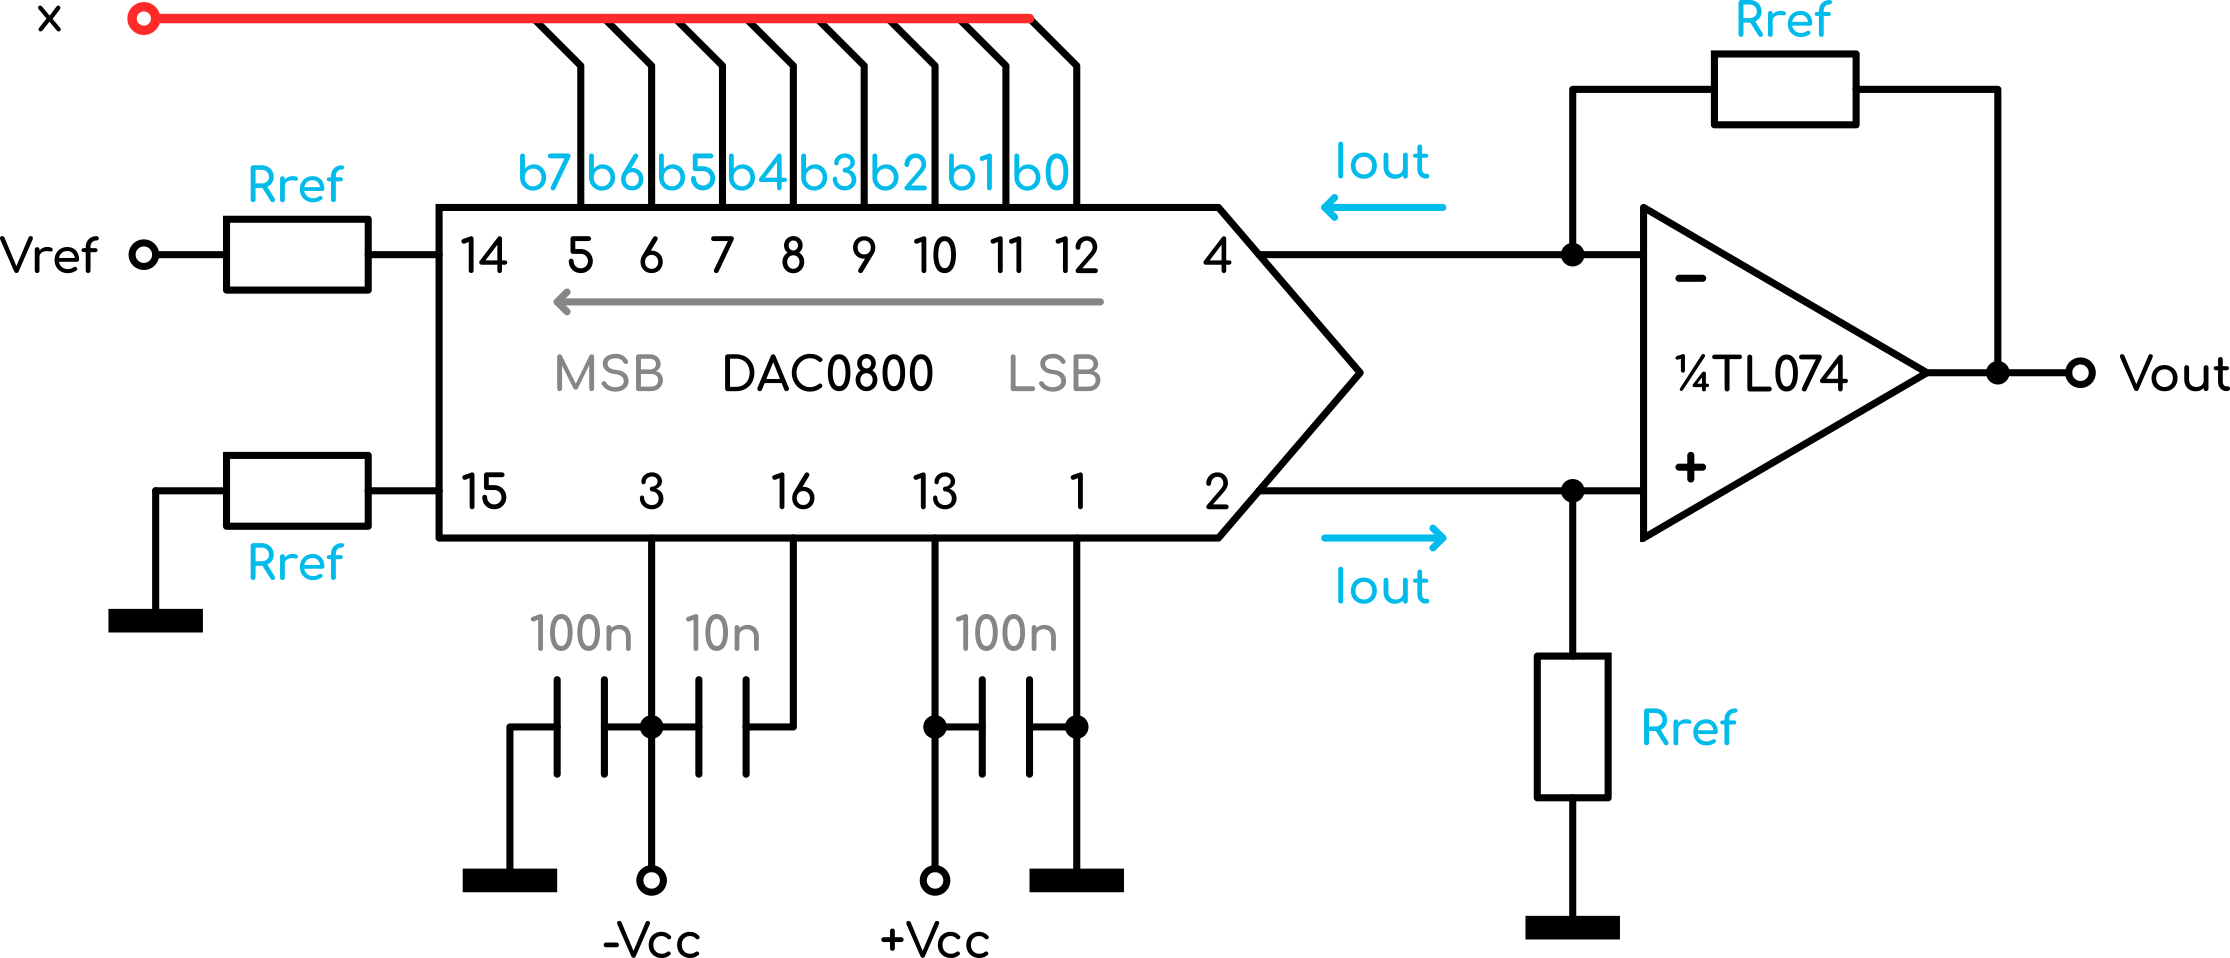
\includegraphics{circuits/DAC_circuit.png}
    \caption{Schema elettrico del DAC, $\pm V_{cc}=\pm 12V$}
    \label{DAC_circuit}
\end{figure}

Il DAC eroga una corrente $I_{out}$ proporzionale all'ingresso digitale $x$, che viene poi
convertita in una tensione con un operazionale. Le due grandezze sono legate dalla seguente
relazione:

\begin{displaymath}
    V_{out}=V_{ref}\left(\frac{2x-255}{256}\right)=5\left(\frac{2x-255}{256}\right)[V]
\end{displaymath}

Il contatore invece viene collegato nel seguente modo:
\medskip

\begin{figure}[ht]
    \centering
    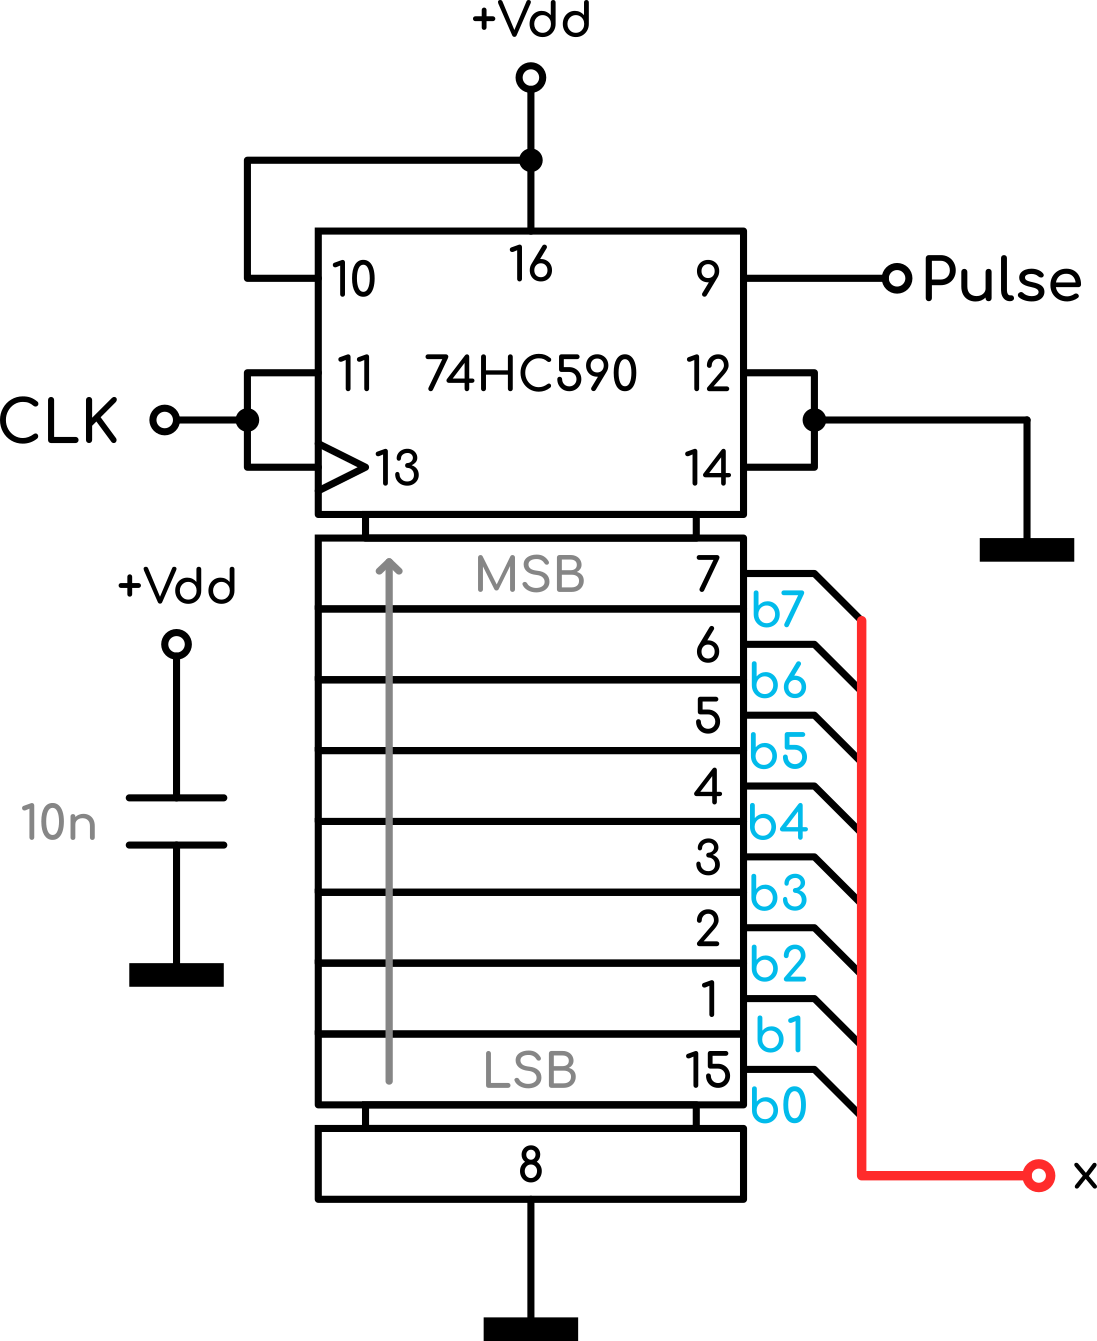
\includegraphics{circuits/ramp_counter_circuit.png}
    \caption{Schema elettrico del contatore per l'onda a rampa, $V_{dd}=+5V$}
    \label{ramp_counter_circuit}
\end{figure}

Si noti l'uscita "Pulse" in figura \ref{ramp_counter_circuit} dalla quale viene prelevato
il segnale a impulso precedentemente accennato, discusso più in dettaglio nel capitolo.
%\ref{ch_impulso}.

Collegando i due blocchi insieme quindi, l'andamento di $V_{out}$ sarà simile a quello
rappresentato in figura \ref{high_res_ramp}, e ad ogni impulso di clock corrisponderà un
gradino di tensione di circa $40mV$ come calcolato precendentemente.

%--------------------------------------------------------------------------------------------

\subsection*{Risultati Pratici}

%--------------------------------------------------------------------------------------------

Andiamo ora a verificare la correttezza del circuito realizzato. Il setup di misura è il
seguente:
\medskip

\begin{figure}[ht]
    \centering
    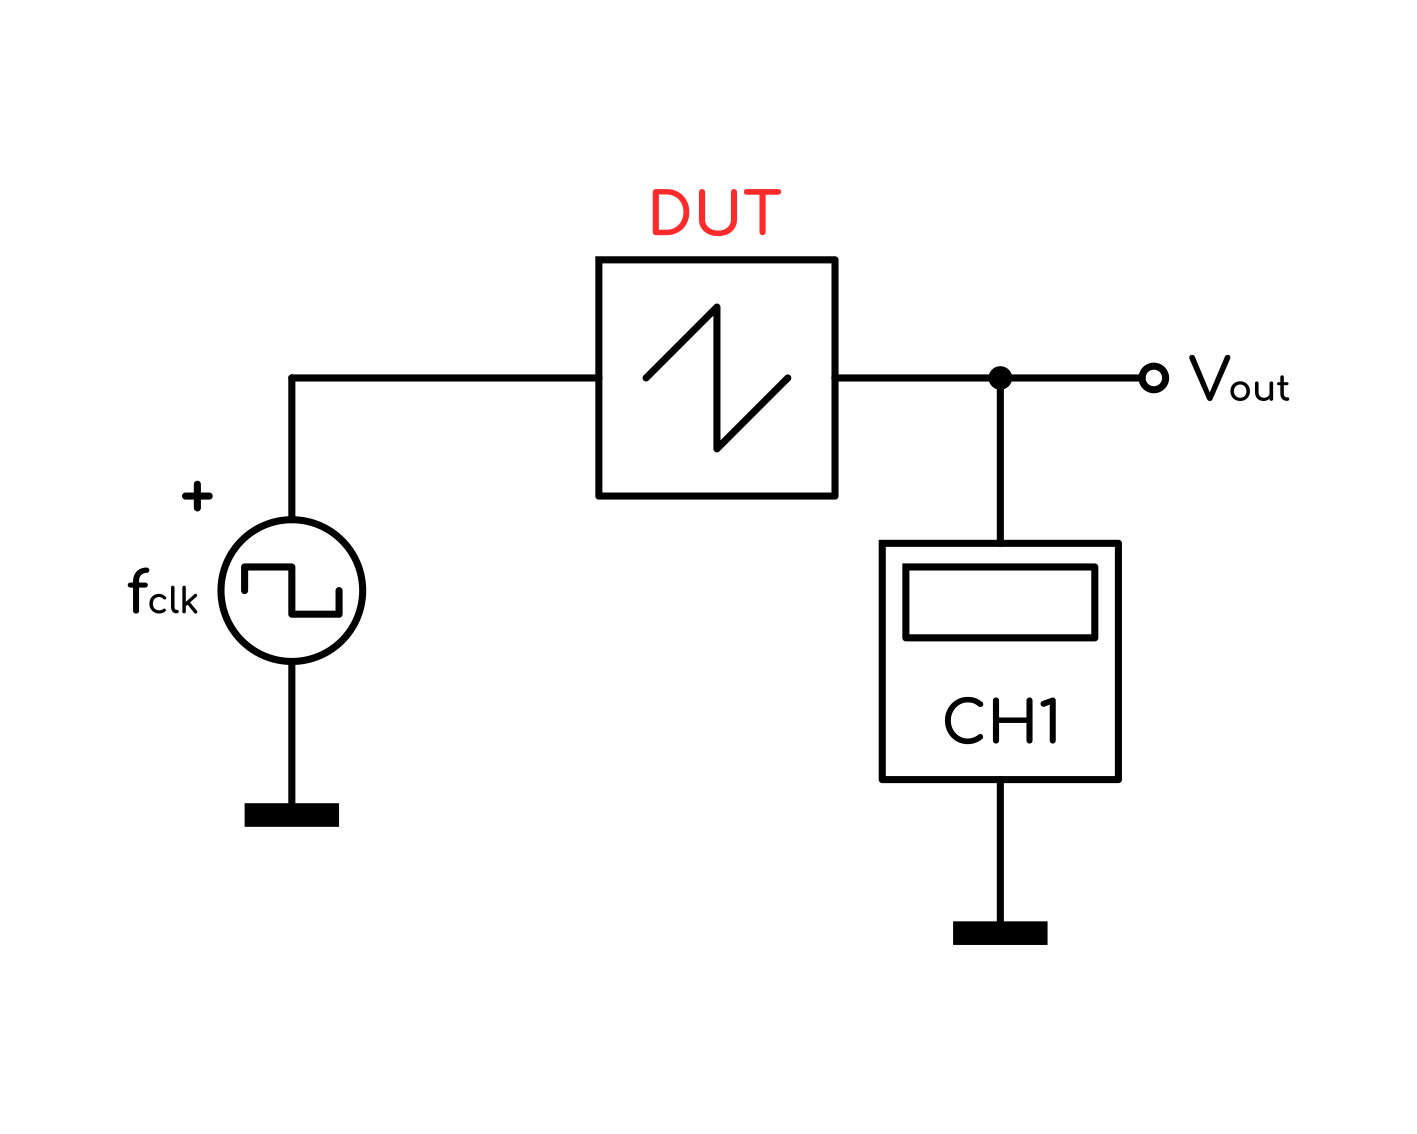
\includegraphics{block_diagrams/mis_ramp.png}
    \caption{Circuito di misura del segnale rampa}
    \label{mis_ramp}
\end{figure}

Si osservano le seguenti forme d'onda:
\medskip

\begin{figure}[ht]
    \centering

    \begin{subfigure}{.5\textwidth}
        \centering
        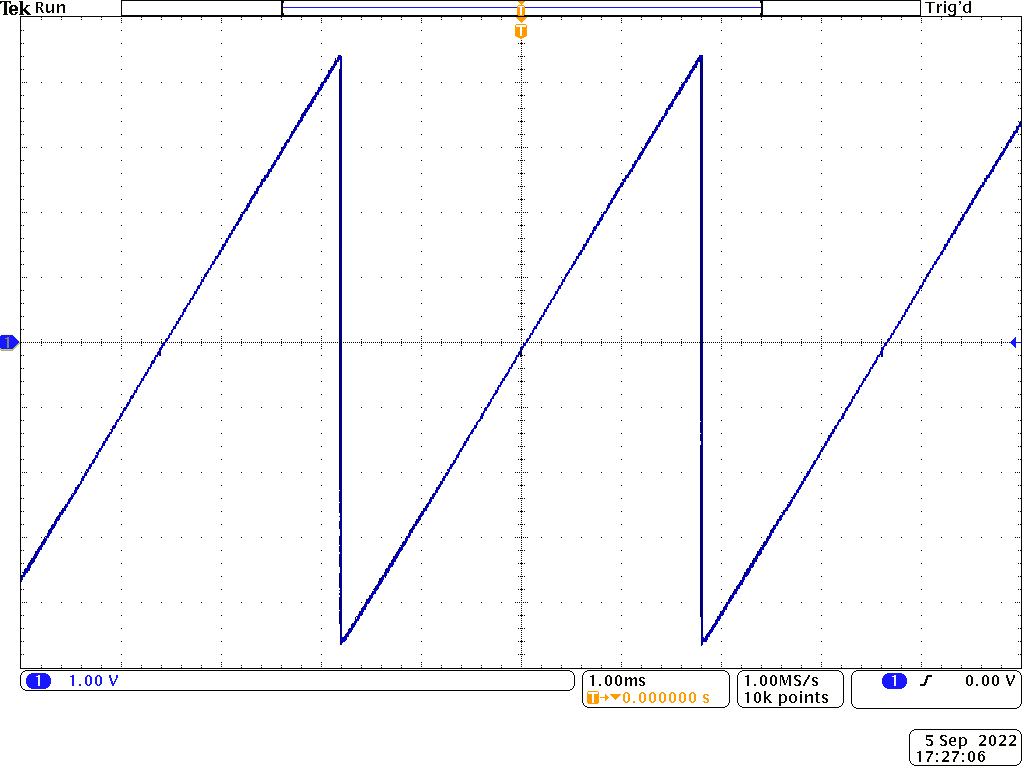
\includegraphics[scale = 0.2]{acquisitions/ramp_wave.png}
        \caption{Acquisizione del segnale a rampa reale}
        \label{acq_ramp}
    \end{subfigure}%
    \begin{subfigure}{.5\textwidth}
        \centering
        
\includegraphics{misc/oscilloscope_placeholder.png}
        \caption{Zoom degli step della rampa acquisita e clock}
        \label{acq_ramp_steps}
    \end{subfigure}

    \caption{Acquisizioni del segnale a rampa}
    \label{acq_ramp_signals}
\end{figure}

%--------------------------------------------------------------------------------------------

\section{Triangolo}

%--------------------------------------------------------------------------------------------

\subsection*{Principio di Funzionamento}

%--------------------------------------------------------------------------------------------

Il ragionamento è del tutto analogo a quello del contatore per la rampa, tuttavia in questo
caso il contatore utilizzato è bidirezionale e necessita di un segnale che determini la
direzione di conteggio (up o down).
\medskip

\begin{figure}[ht]
    \centering
    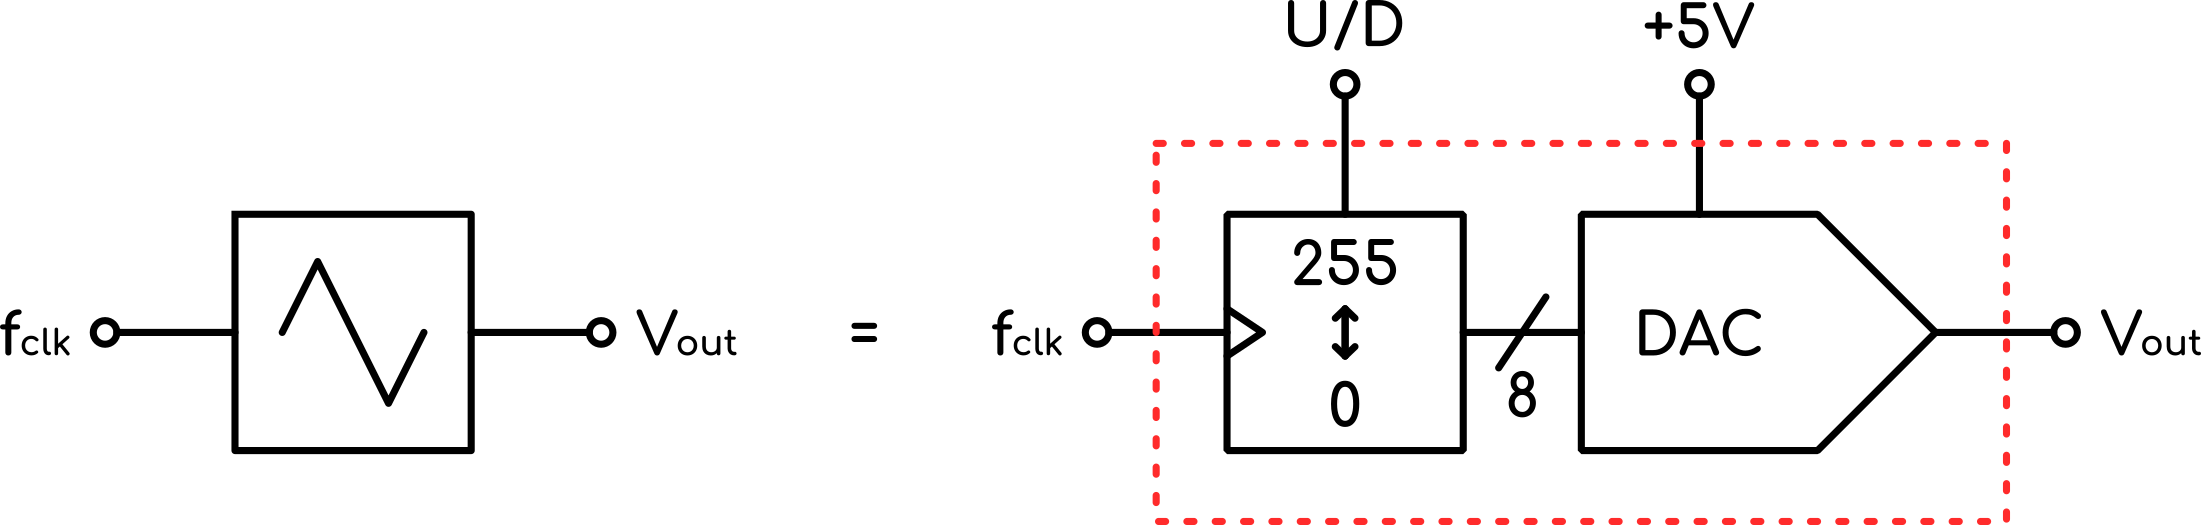
\includegraphics{block_diagrams/triangle_block_diagram.png}
    \caption{Schema a blocchi del sottosistema per la generazione del triangolo}
    \label{triangle_block_diagram}
\end{figure}

\begin{figure}[ht]
    \centering

    \begin{subfigure}{.5\textwidth}
        \centering
        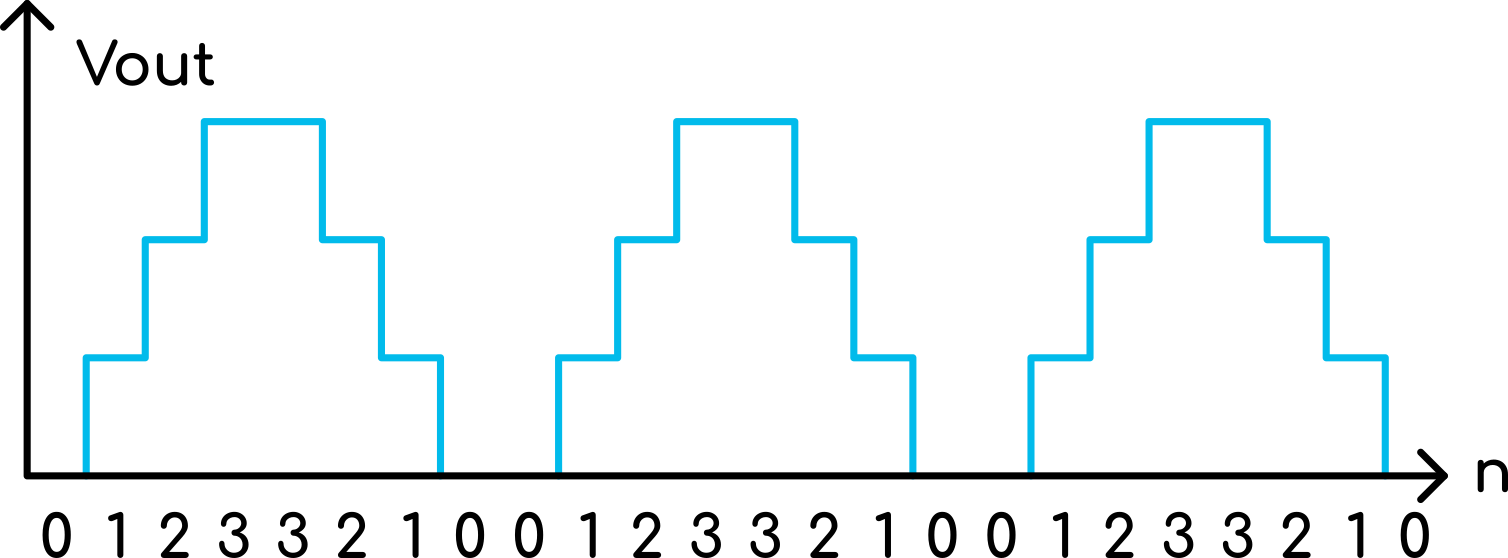
\includegraphics{graphs/low_res_triangle.png}
        \caption{Triangolo ottenuto con un contatore a 2 bit}
        \label{low_res_triangle}
    \end{subfigure}%
    \begin{subfigure}{.5\textwidth}
        \centering
        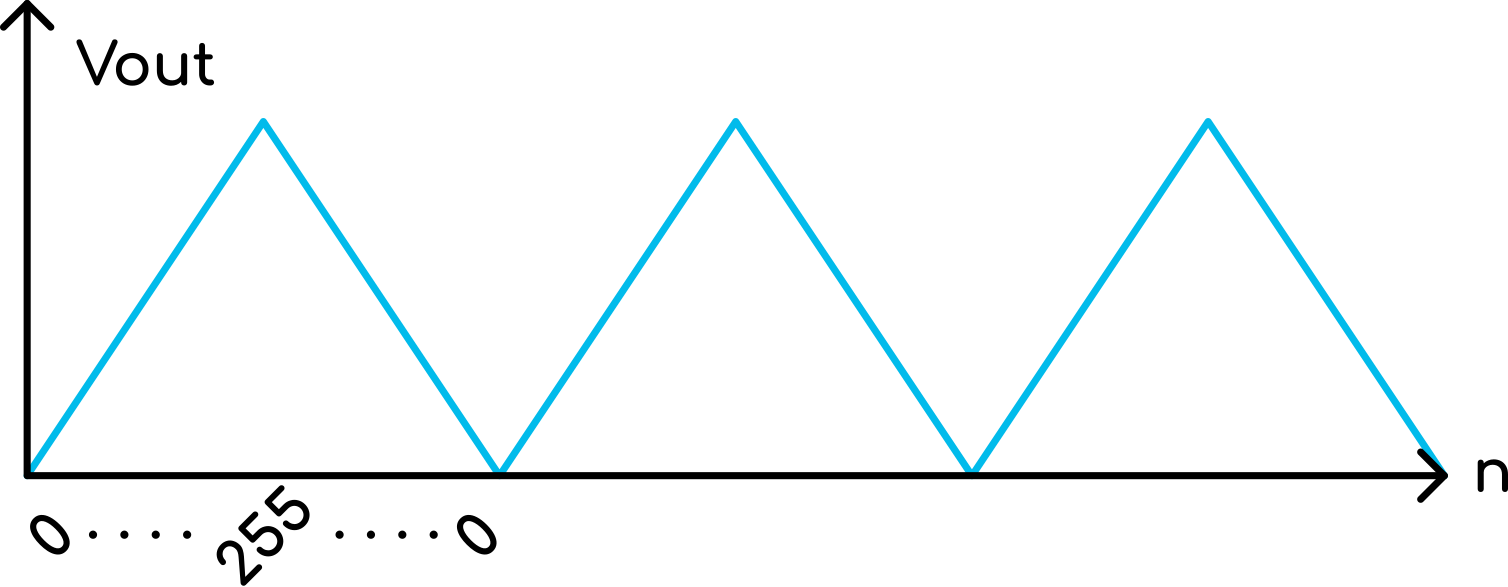
\includegraphics{graphs/high_res_triangle.png}
        \caption{Triangolo ottenuto con un contatore a 8 bit}
        \label{high_res_triangle}
    \end{subfigure}

    \caption{Confronto tra contatori bidirezionali con diverso numero di bit}
    \label{triangles}
\end{figure}

La configurazione del DAC rimane quella utilizzata per la rampa, rappresentata in figura
\ref{DAC_circuit}, va tuttavia fatta notare una importante differenza, ovvero che in questo
caso il numero di cicli di clock utilizzati è doppio rispetto a quello per la rampa. Infatti
dovranno essere eseguiti 256 conteggi verso l'alto e 256 conteggi verso il basso per effettuare
un singolo periodo di onda triangolare. Ne consegue quindi che anche la frequenza di clock
in ingresso a questo sottosistema dovrà essere doppia rispetto alla rampa, come risulta
evidente in figura \ref{steps}.
\medskip

\begin{figure}[ht]
    \centering

    \begin{subfigure}{.5\textwidth}
        \centering
        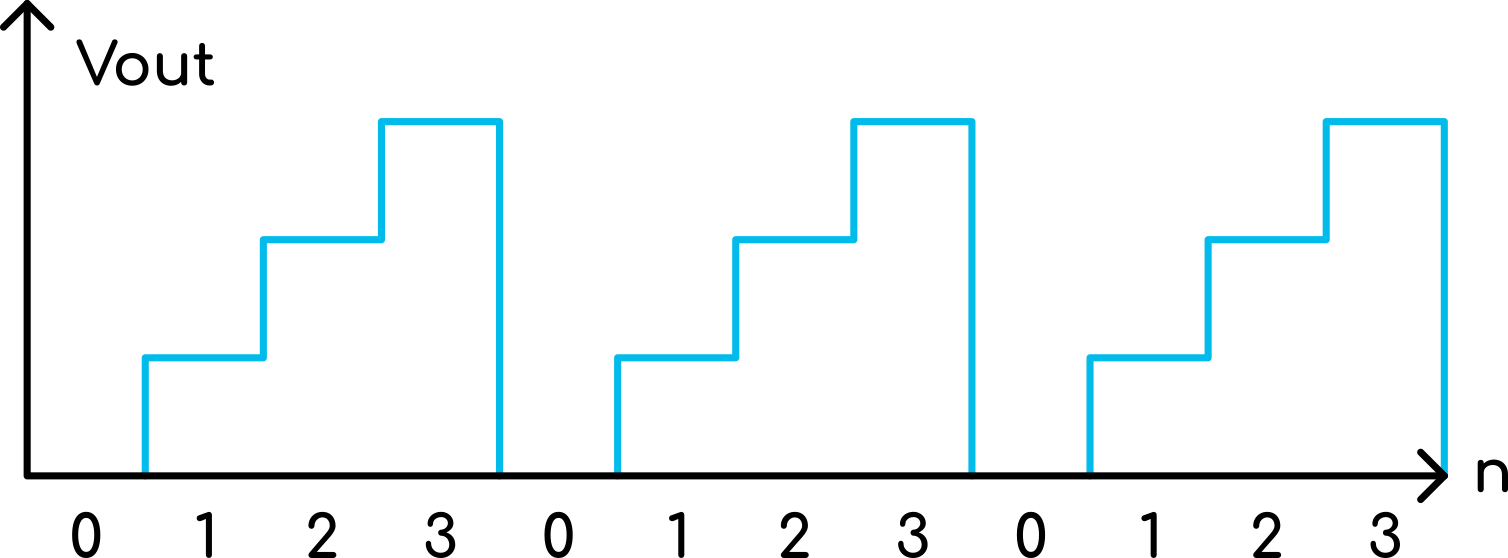
\includegraphics{graphs/low_res_ramp.png}
        \caption{Rampa ottenuta con un contatore a 2 bit}
    \end{subfigure}%
    \begin{subfigure}{.5\textwidth}
        \centering
        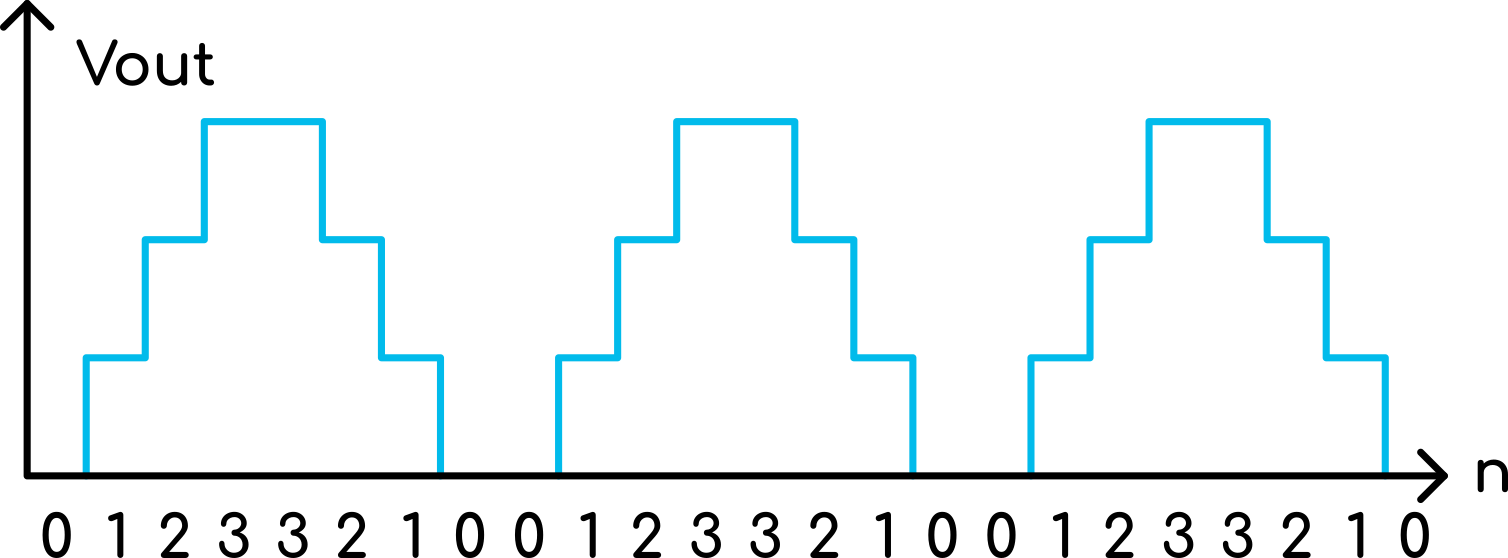
\includegraphics{graphs/low_res_triangle.png}
        \caption{Triangolo ottenuto con un contatore a 2 bit}
    \end{subfigure}

    \caption{Confronto del conteggio tra contatori unidirezionali e bidirezionali}
    \label{steps}
\end{figure}

%--------------------------------------------------------------------------------------------

\subsection*{Componenti Utilizzati e Schemi Elettrici}

%--------------------------------------------------------------------------------------------

L'unico componente diverso rispetto al circuito per la rampa è il contatore, che come già
detto deve essere bidirezionale. Si utilizzano due 74LS169 \cite{74ls169} in cascata con
la seguente configurazione:
\medskip

\begin{figure}[ht]
    \centering
    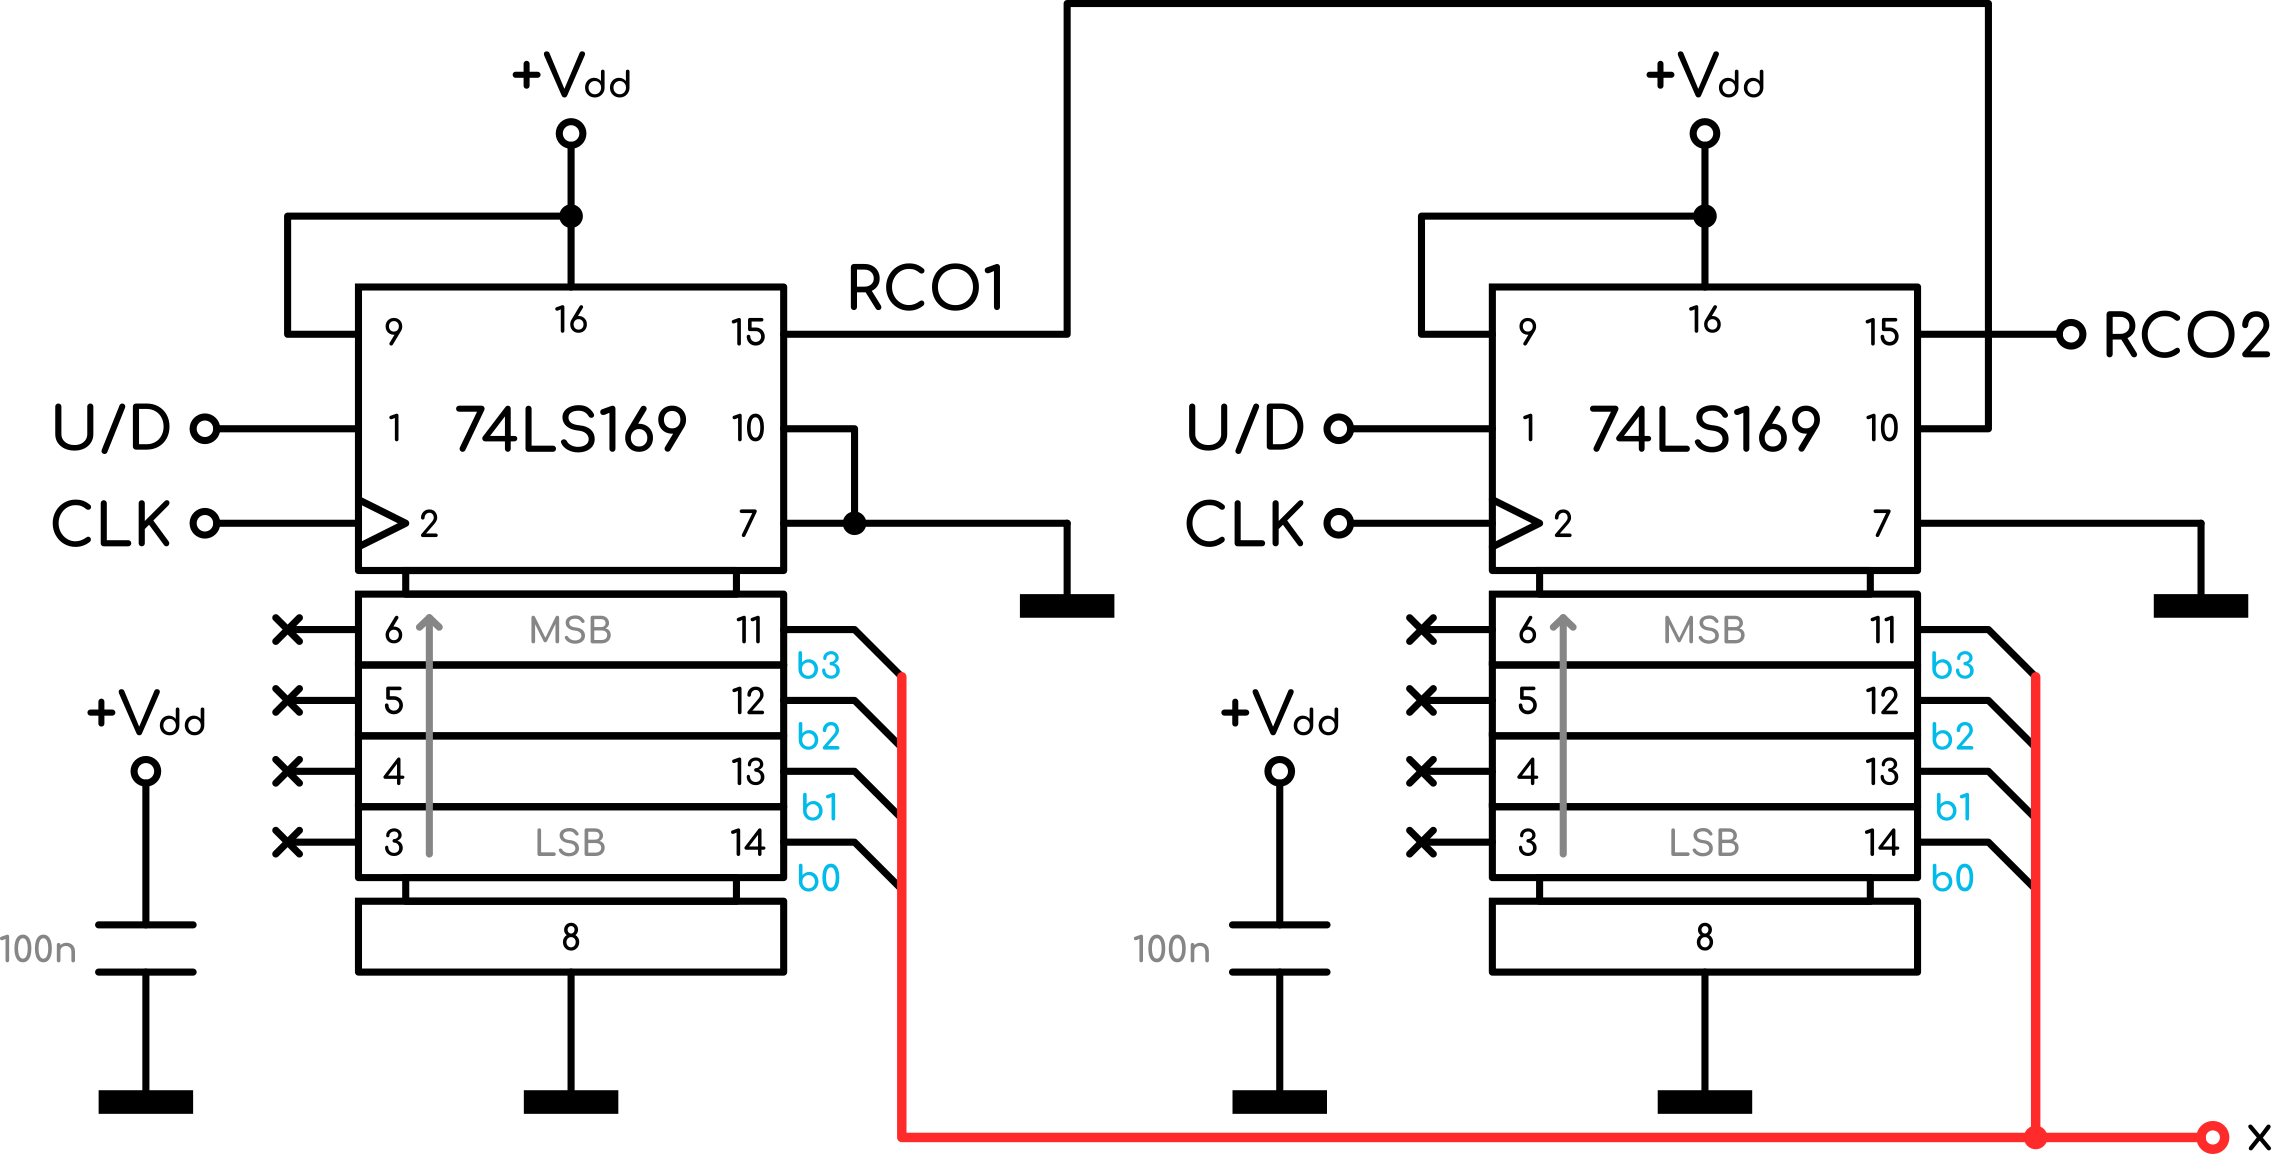
\includegraphics{circuits/triangle_counter_circuit.png}
    \caption{Schema elettrico dei contatori per l'onda triangolare, $V_{dd}=+5V$}
    \label{triangle_counter_circuit}
\end{figure}

Il componente utilizzato presenta anche degli ingressi per il preset del numero di partenza
(pin da 3 a 6), che però nel nostro caso non vengono utilizzati.

L'uscita denominata $RCO2$ verrà utilizzata per pilotare il verso del conteggio.

%--------------------------------------------------------------------------------------------

\subsection*{Risultati Pratici}

%--------------------------------------------------------------------------------------------

Andiamo ora a verificare la correttezza del circuito realizzato. Il setup di misura è il
seguente:
\medskip

\begin{figure}[ht]
    \centering
    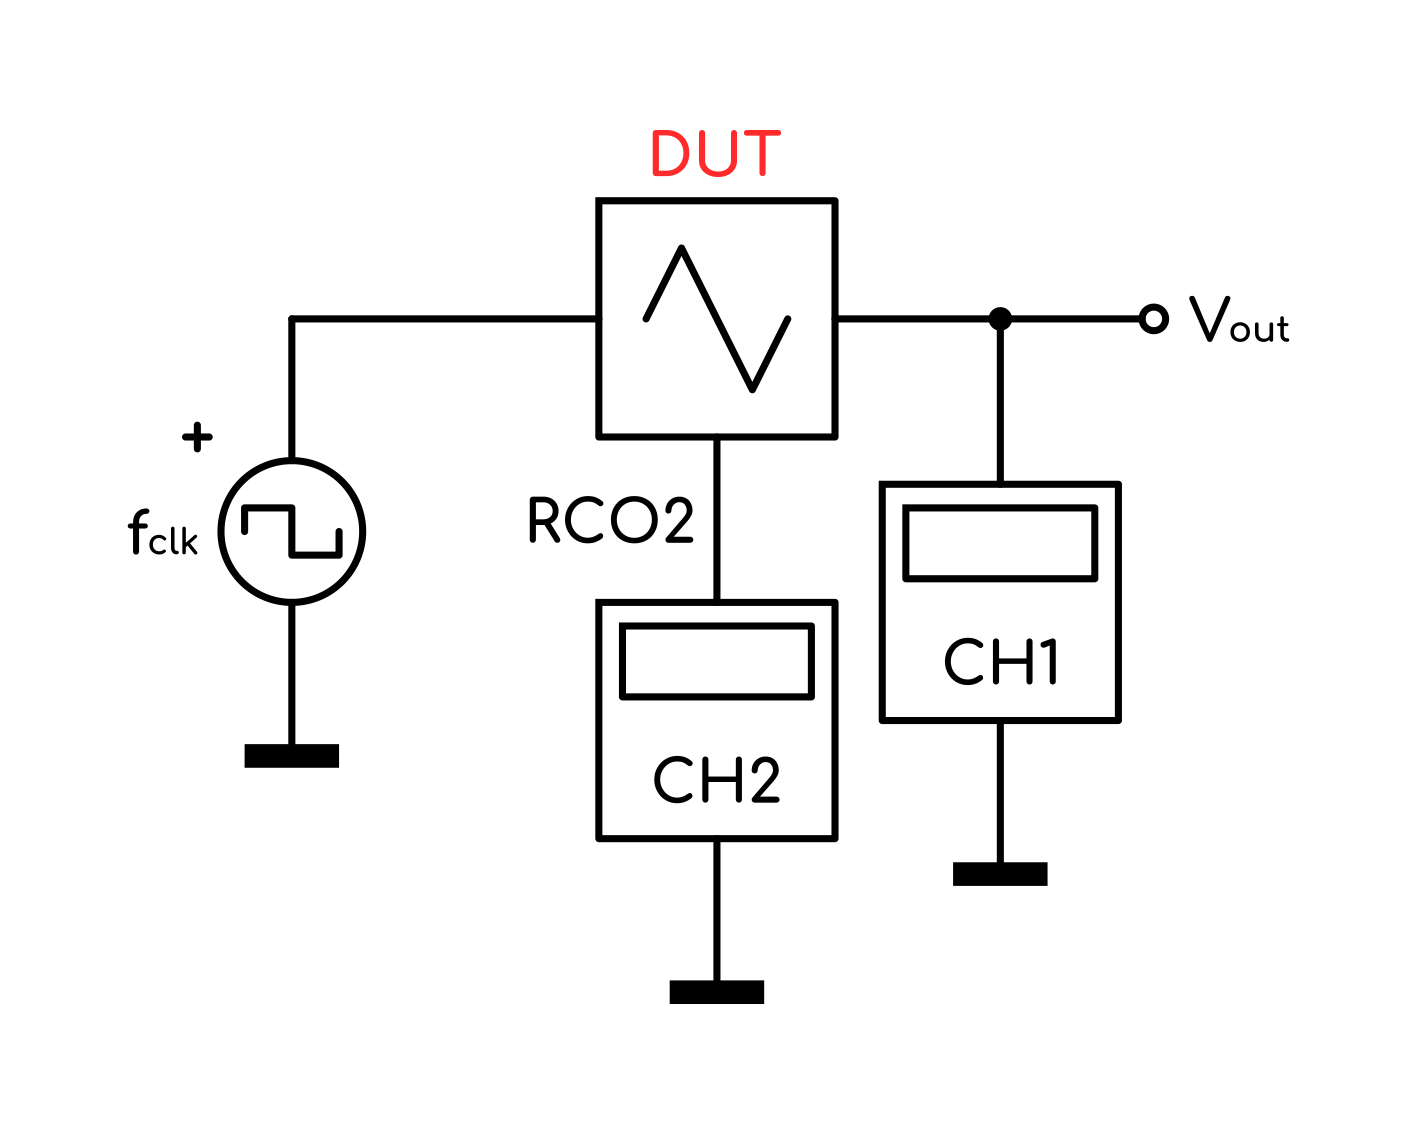
\includegraphics{block_diagrams/mis_triangle.png}
    \caption{Circuito di misura del segnale triangolo}
    \label{mis_triangle}
\end{figure}

Si osservano le seguenti forme d'onda:
\medskip

\begin{figure}[ht]
    \centering

    \begin{subfigure}{.5\textwidth}
        \centering
        
\includegraphics{misc/oscilloscope_placeholder.png}
        \caption{Acquisizione del segnale a triangolo reale}
        \label{acq_triangle}
    \end{subfigure}%
    \begin{subfigure}{.5\textwidth}
        \centering
        
\includegraphics{misc/oscilloscope_placeholder.png}
        \caption{Zoom degli step del triangolo acquisito e clock}
        \label{acq_triangle_steps}
    \end{subfigure}

    \caption{Acquisizioni del segnale a triangolo}
    \label{acq_triangle_signals}
\end{figure}

%--------------------------------------------------------------------------------------------

\section{Adattamento dei Segnali di Clock}

%--------------------------------------------------------------------------------------------

Si è visto come, per avere la stessa frequenza di segnale d'uscita, il contatore del
triangolo deve avere una frequenza di clock doppia rispetto a quella del contatore della
rampa. Questo problema si risolve facilmente utilizzando un divisore di frequenza,
ottenuto con un semplice toggle flip-flop (TFF).
\medskip

\begin{figure}[ht]
    \centering
    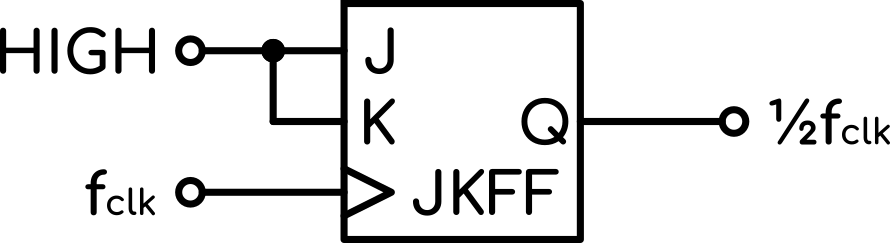
\includegraphics{block_diagrams/freq_divider_block_diagram.png}
    \caption{Schema a blocchi del divisore di frequenza}
    \label{freq_divider_block_diagram}
\end{figure}

Le specifiche sul segnale di clock ci impongono allora di generare un segnale a onda quadra
con frequenza variabile tra $\approx14kHz$ e $\approx3.6MHz$.

Invece, per fare in modo che il contatore del triangolo cambi effettivamente verso di conteggio
è necessario utilizzare un altro TFF collegato al segnale $RCO2$ invertito (poichè attivo a
livello logico basso) e all'ingresso $U/D$.
\medskip

\begin{figure}[ht]
    \centering
    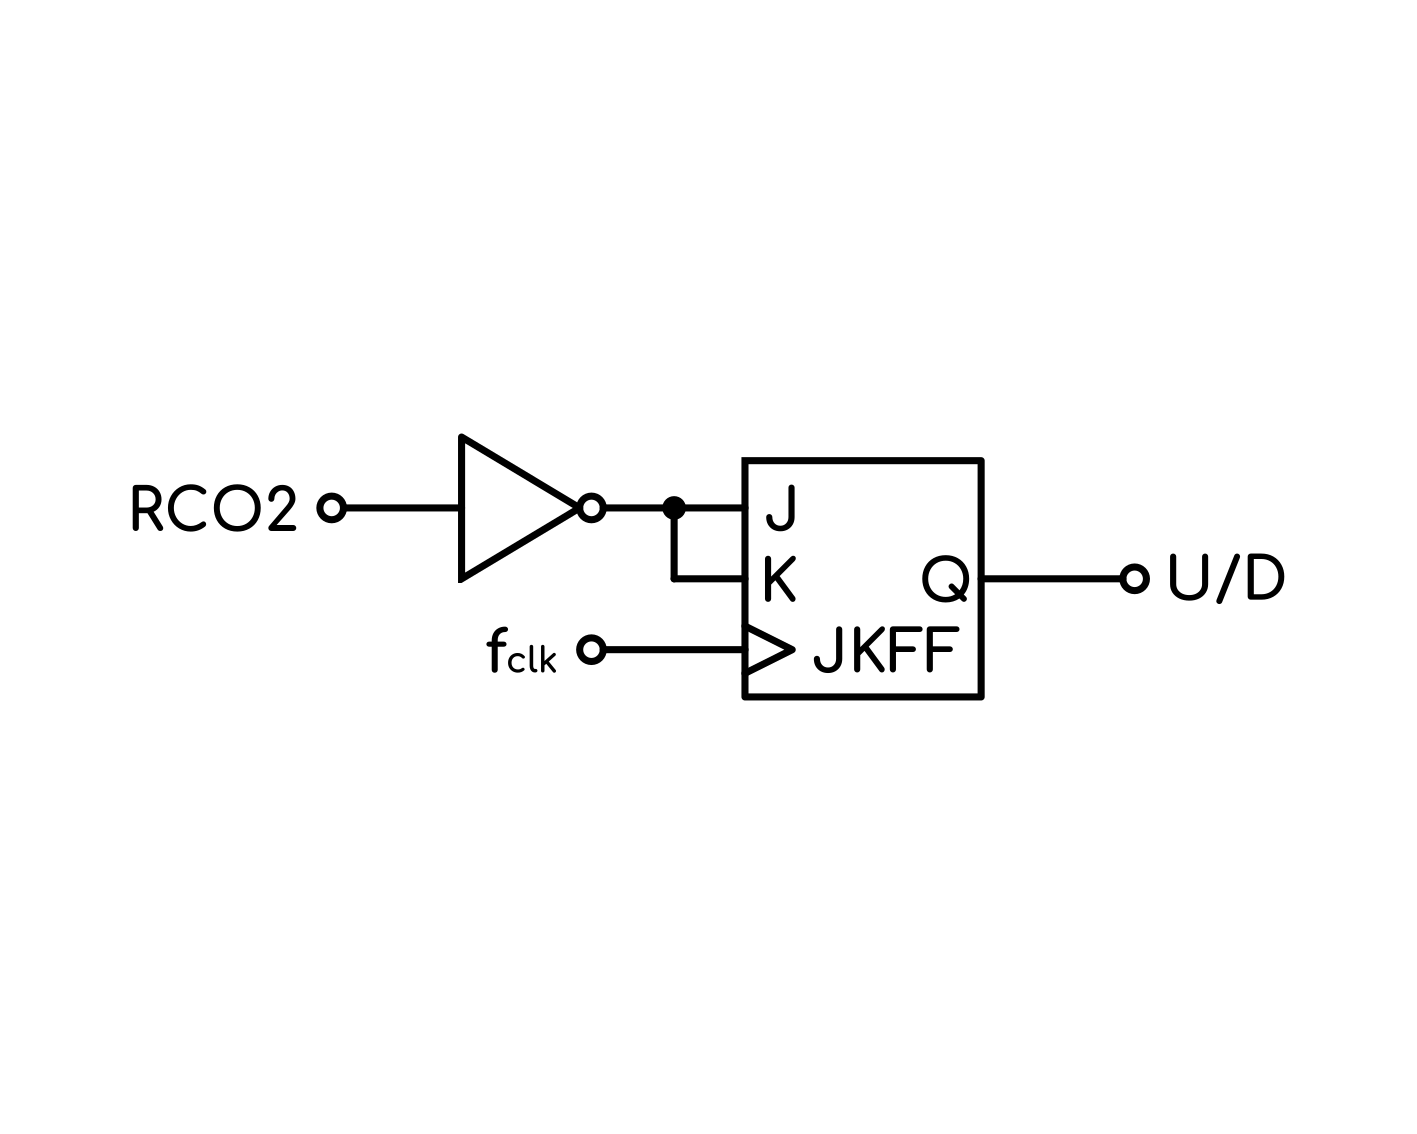
\includegraphics{block_diagrams/UD_block_diagram.png}
    \caption{Schema a blocchi del sistema per il segnale di pilotaggio}
    \label{UD_block_diagram}
\end{figure}

I componenti utilizzati per questo scopo sono:

\begin{itemize}
    \item Flip-Flop: 74HC73 \cite{74hc73};
    \item MOSFET: 2N7000 \cite{2n7000};
\end{itemize}

Il chip utilizzato per i flip-flop fornisce esattamente le 2 unità necessarie al nostro
scopo, mentre lo schema elettrico per l'inverter è rappresentato in figura
\ref{inverter_circuit}, dove il MOSFET utilizzato è compatibile con le tensioni logiche
presenti nel circuito.
\medskip

\begin{figure}[ht]
    \centering
    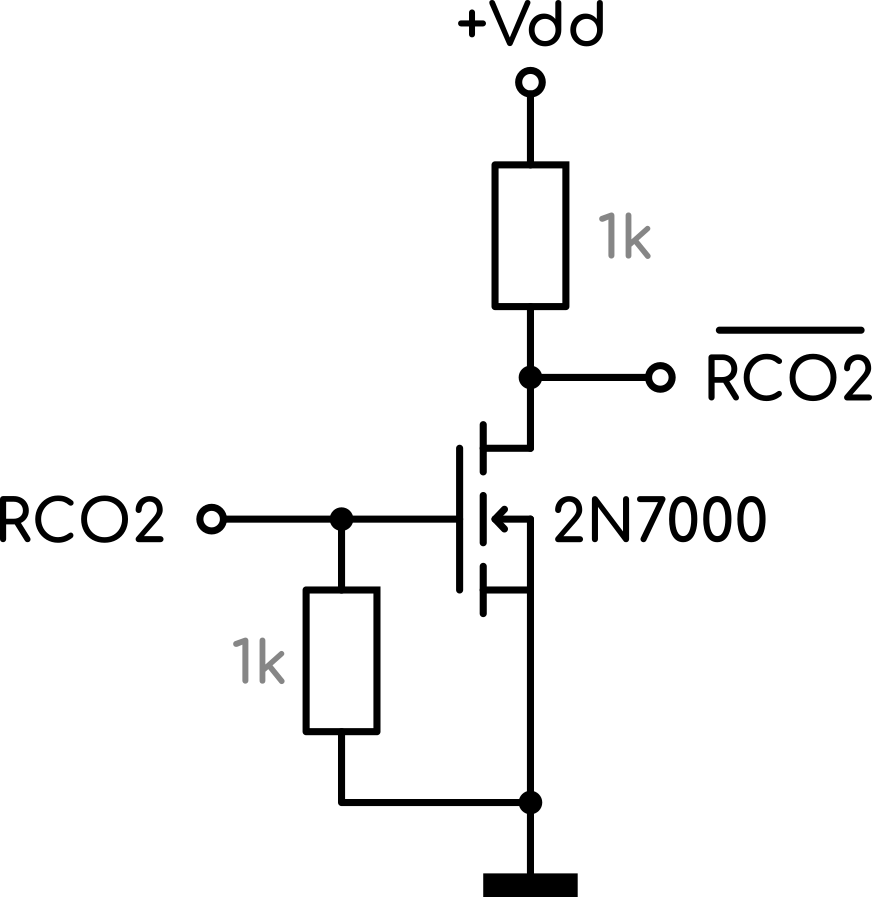
\includegraphics{circuits/inverter_circuit.png}
    \caption{Schema elettrico dell'inverter logico, $V_{dd}=+5V$}
    \label{inverter_circuit}
\end{figure}

%--------------------------------------------------------------------------------------------

\subsection*{Risultati Pratici}

%--------------------------------------------------------------------------------------------

Si verifica la correttezza dei circuiti:
\medskip

\begin{figure}[ht]
    \centering

    \begin{subfigure}{.5\textwidth}
        \centering
        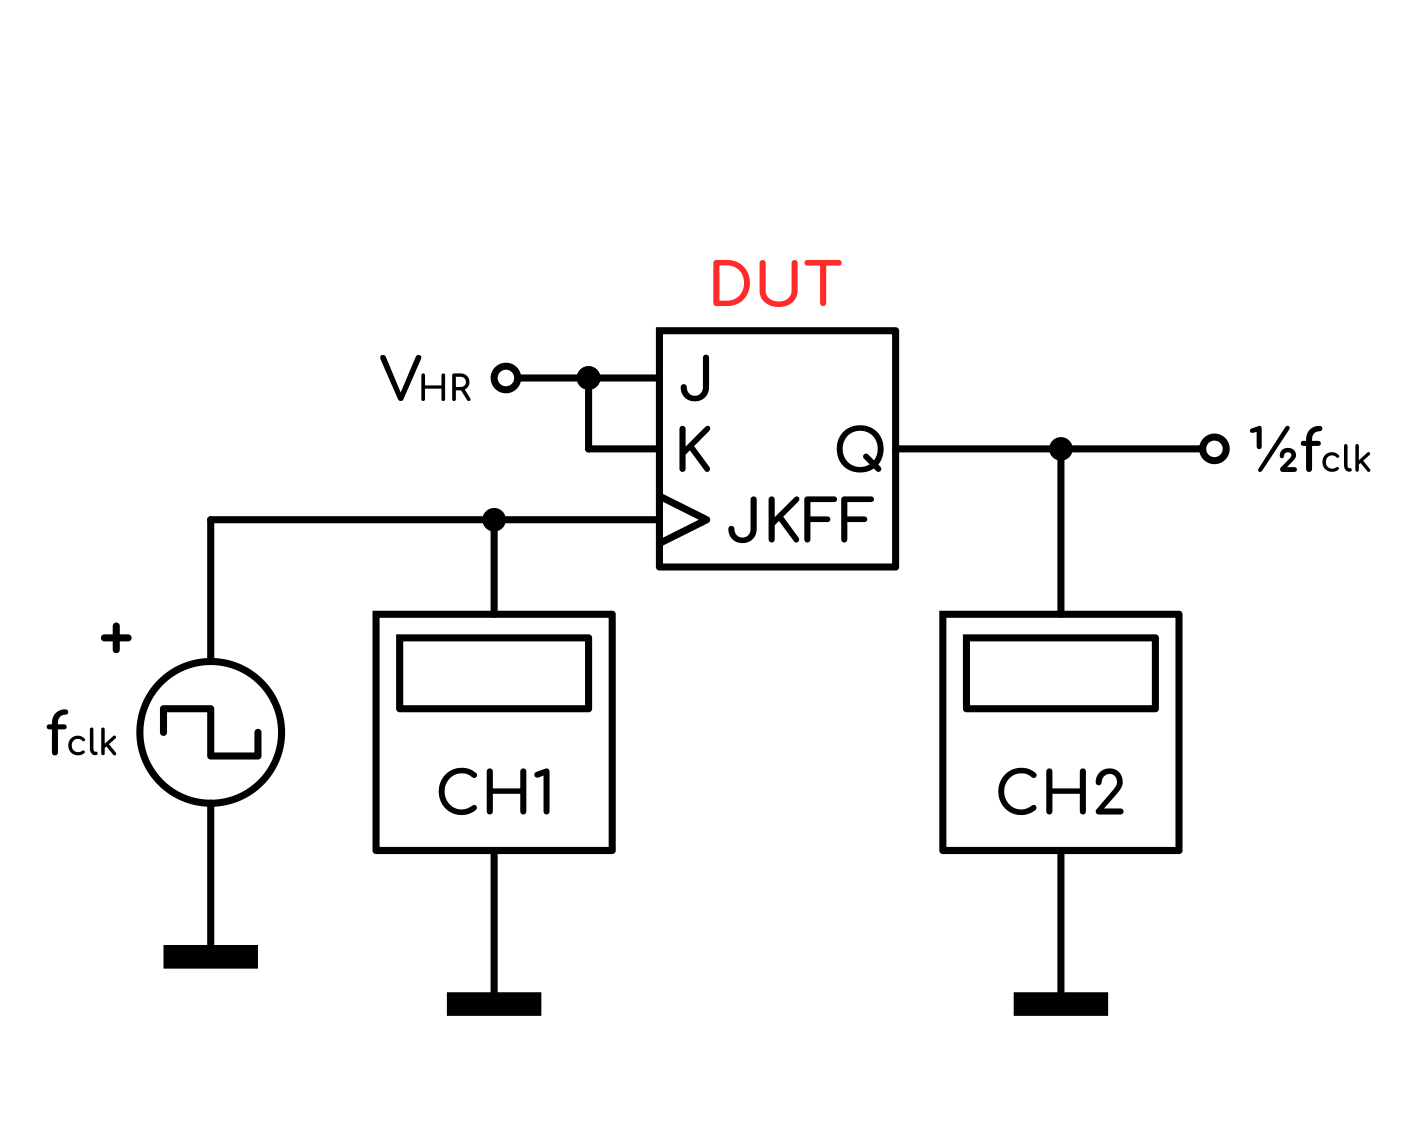
\includegraphics{block_diagrams/mis_clock_divider.png}
        \caption{Circuito di misura del divisore di frequenza}
        \label{mis_clock_divider}
    \end{subfigure}%
    \begin{subfigure}{.5\textwidth}
        \centering
        
\includegraphics{misc/oscilloscope_placeholder.png}
        \caption{Acquisizione dei segnali $f_{clk}$ e $f_{clk}/2$}
        \label{acq_clock_divider}
    \end{subfigure}

    \caption{Correttezza del circuito divisore di frequenza}
    \label{clock_divider}
\end{figure}

\begin{figure}[ht]
    \centering

    \begin{subfigure}{.5\textwidth}
        \centering
        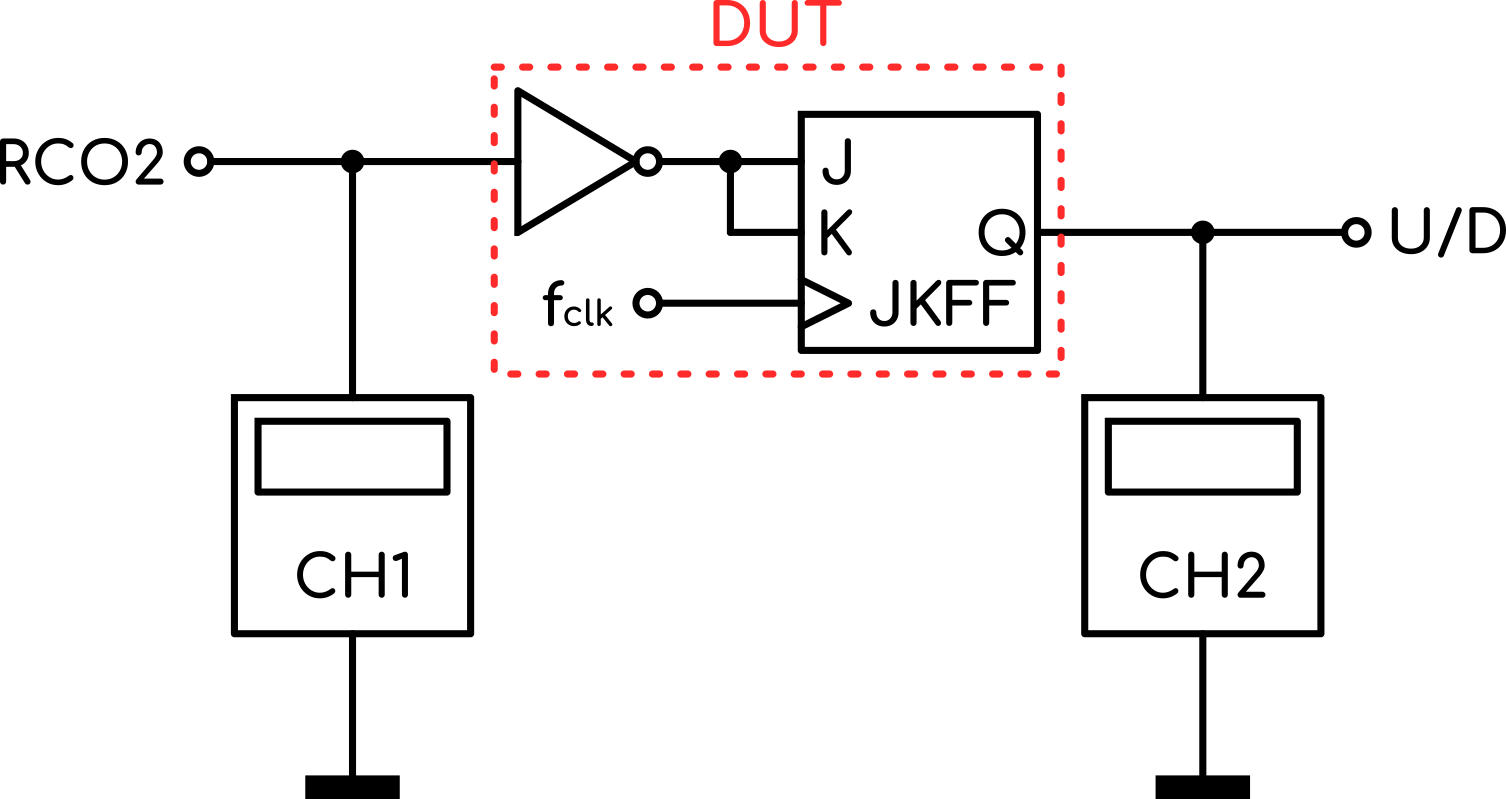
\includegraphics{block_diagrams/mis_UD.png}
        \caption{Circuito di misura del segnale $U/D$}
        \label{mis_UD}
    \end{subfigure}%
    \begin{subfigure}{.5\textwidth}
        \centering
        
\includegraphics{misc/oscilloscope_placeholder.png}
        \caption{Acquisizione dei segnali $RCO2$ e $U/D$}
        \label{acq_UD}
    \end{subfigure}

    \caption{Correttezza del circuito di pilotaggio del contatore up-down}
    \label{UD}
\end{figure}
\chapter{Convertitore Tensione-Frequenza}

%--------------------------------------------------------------------------------------------

Si vuole ora progettare il circuito per la generazione del segnale $f_{clk}$, con le
specifiche ottenute dai capitoli precedenti, ovvero:

\begin{itemize}
    \item Frequenza minima: $\approx 14\ kHz$;
    \item Frequenza massima: $\approx 3.6\ MHz$;
    \item Livello logico basso: $0\ V$;
    \item Livello logico alto: $+5\ V$;
\end{itemize}

%--------------------------------------------------------------------------------------------

\subsection*{Principio di Funzionamento}

%--------------------------------------------------------------------------------------------

Ciò di cui abbiamo bisogno è un circuito in grado di convertire una tensione in un segnale
a onda rettangolare con frequenza proporzionale alla tensione stessa, ovvero un convertitore
tensione-frequenza.

In commercio è possibile trovare diversi chip in grado di svolgere questa funzione
semplicemente aggiungendo una manciata di componenti di contorno, anche se la maggior
parte di questi non arriva a coprire l'intero range di funzionamento di cui abbiamo bisogno
(come ad esempio il noto LM331 \cite{lm331}). Nel nostro caso si utilizza un VFC110
\cite{vfc110}, circuito integrato specializzato che vanta un'ottima linearità e la capacità
di fornire una frequenza massima di $4\ MHz$ in uscita con una corrispondente tensione in
ingresso di $+10\ V$, esattamente ciò che la nostra applicazione richiede.

\begin{figure}[H]
    \centering
    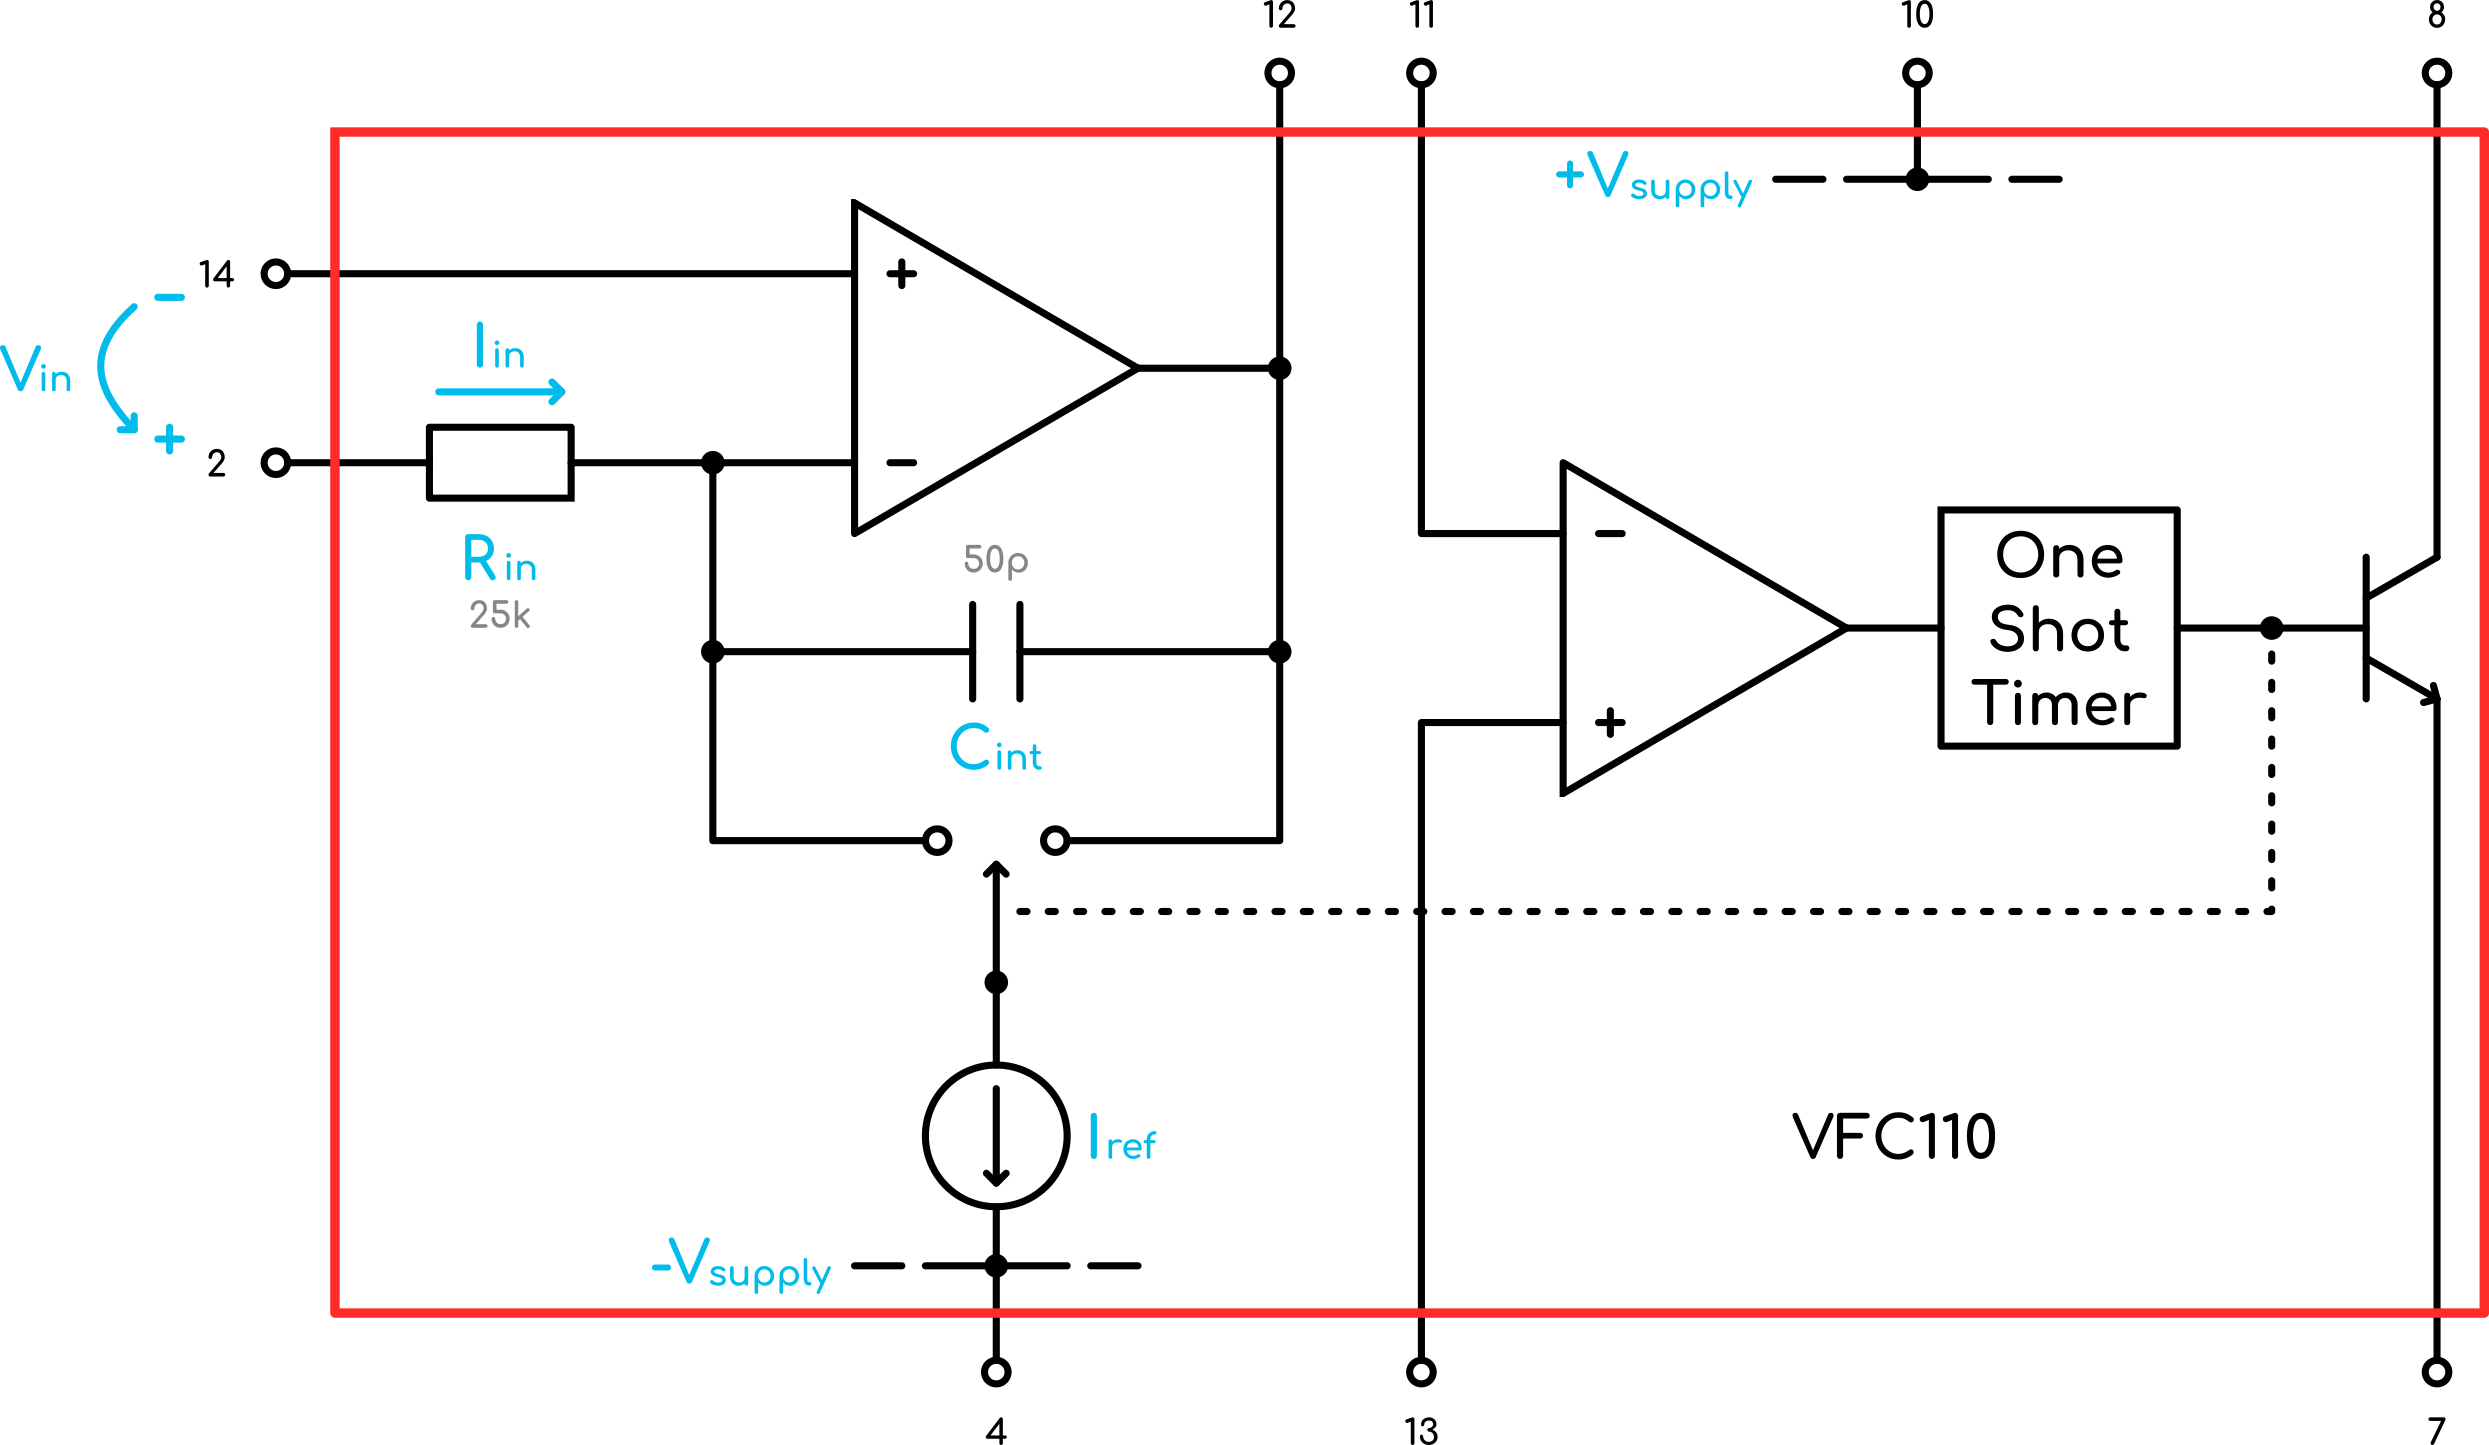
\includegraphics{circuits/vfc110_internal.png}
    \caption{Estratto utile della struttura interna di un VFC110}
    \label{vfc110_internal}
\end{figure}

Il cuore del circuito (figura \ref{vfc110_internal}) consiste in un operazionale configurato
come integratore, con tensione di uscita proporzionale alla carica immagazzinata nella sua
capacità di feedback $C_{int}$. Una tensione in ingresso $V_{in}$ sviluppa una corrente
$I_{in}=\frac{V_{in}}{R_{in}}$ che viene forzata in $C_{int}$, causando quindi una rampa
decrescente in uscita. Arrivati a $0\ V$ il comparatore scatta, attivando il timer one-shot.
Quindi un generatore di corrente $I_{ref}$ (dal valore di circa $1\ mA$) viene connesso
all'ingresso dell'integratore per un periodo di durata pari a $T_{OS}$, causando una rampa
crescente in uscita. Infine il ciclo ricomincia.

\begin{figure}[H]
    \centering
    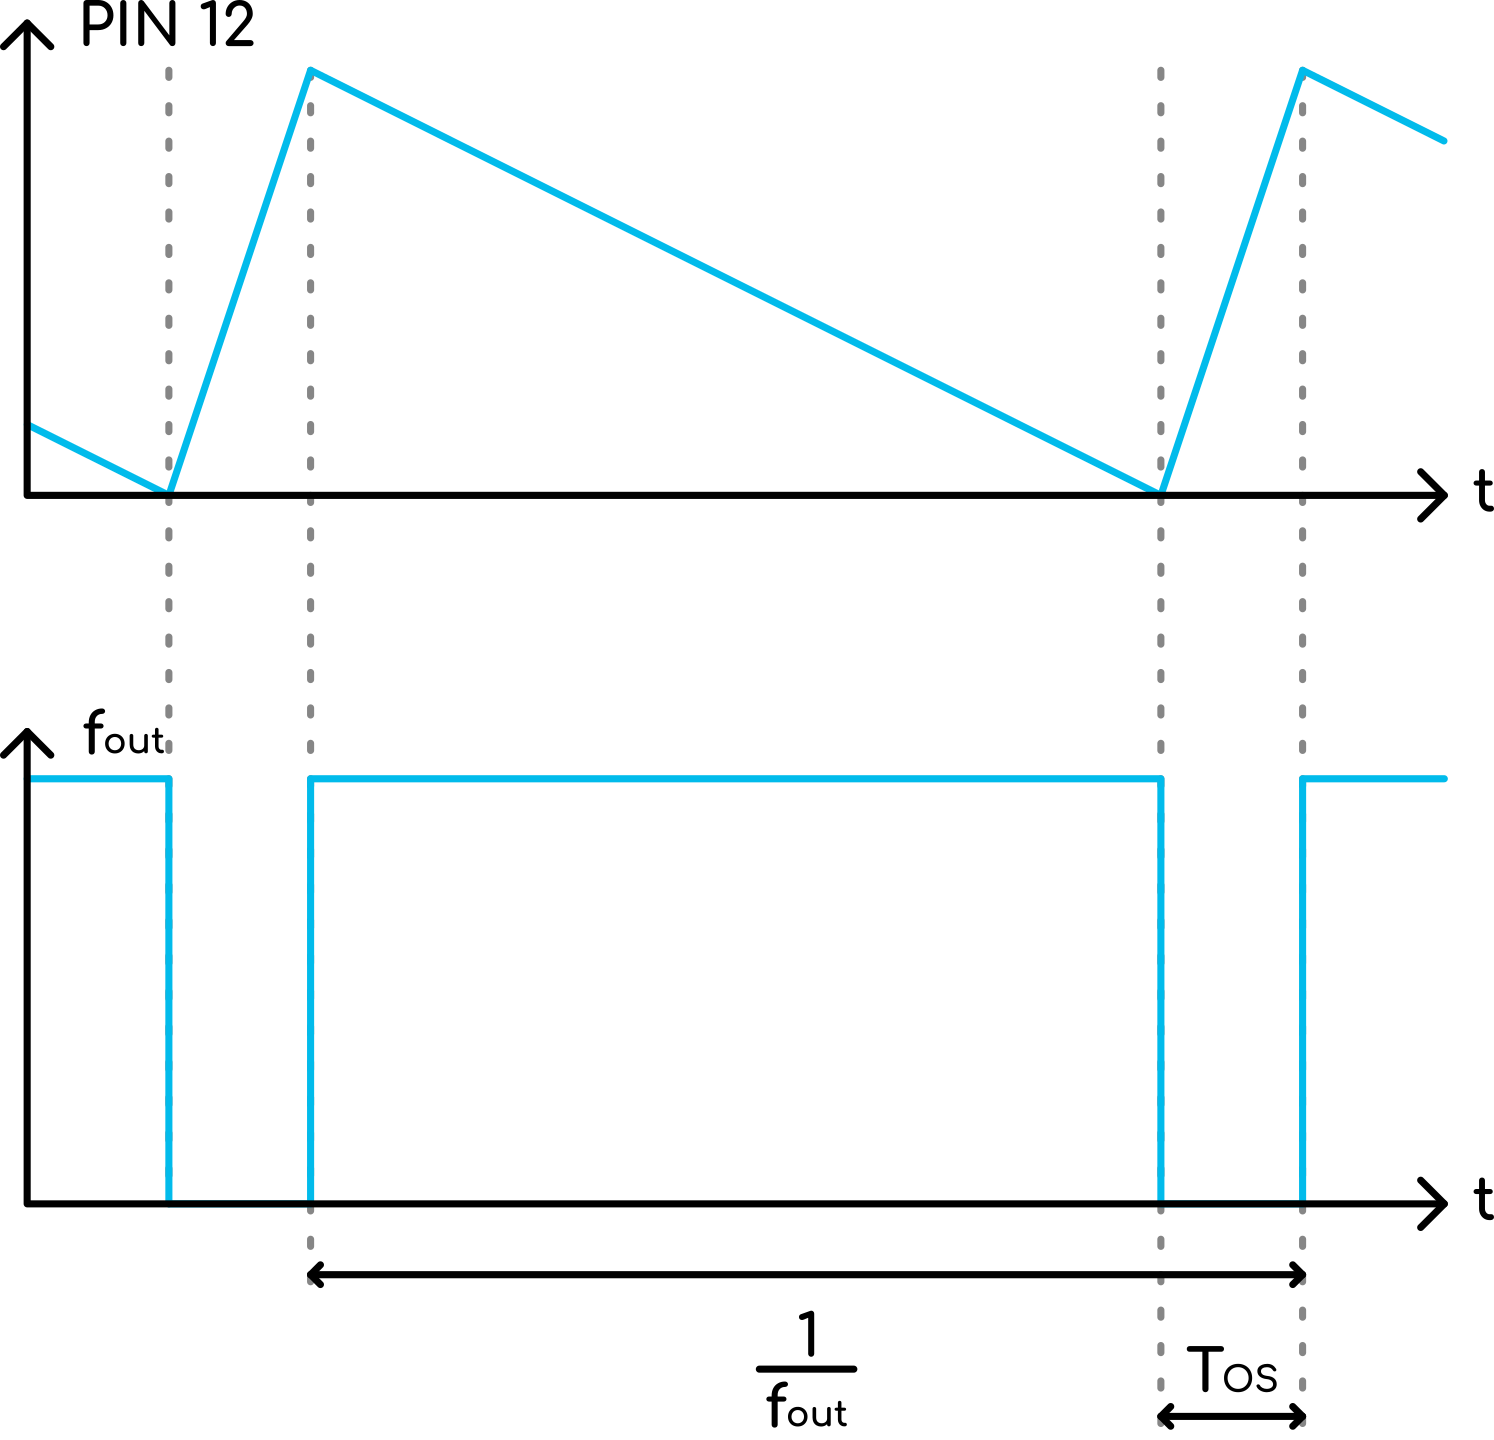
\includegraphics{graphs/integrator_behaviour.png}
    \caption{Forme d'onda teoriche del VFC110}
    \label{integrator_behaviour}
\end{figure}

Per uno studio più approfondito sul funzionamento del VFC110 si consiglia la lettura del
datasheet del componente, dal quale si ricava la configurazione del circuito utilizzato
per sfruttare l'intero range offerto (figura \ref{VFC_circuit}). Si modificano solo i valori
di alimentazione, sostituendoli con quelli dello standard scelto.

\begin{figure}[H]
    \centering
    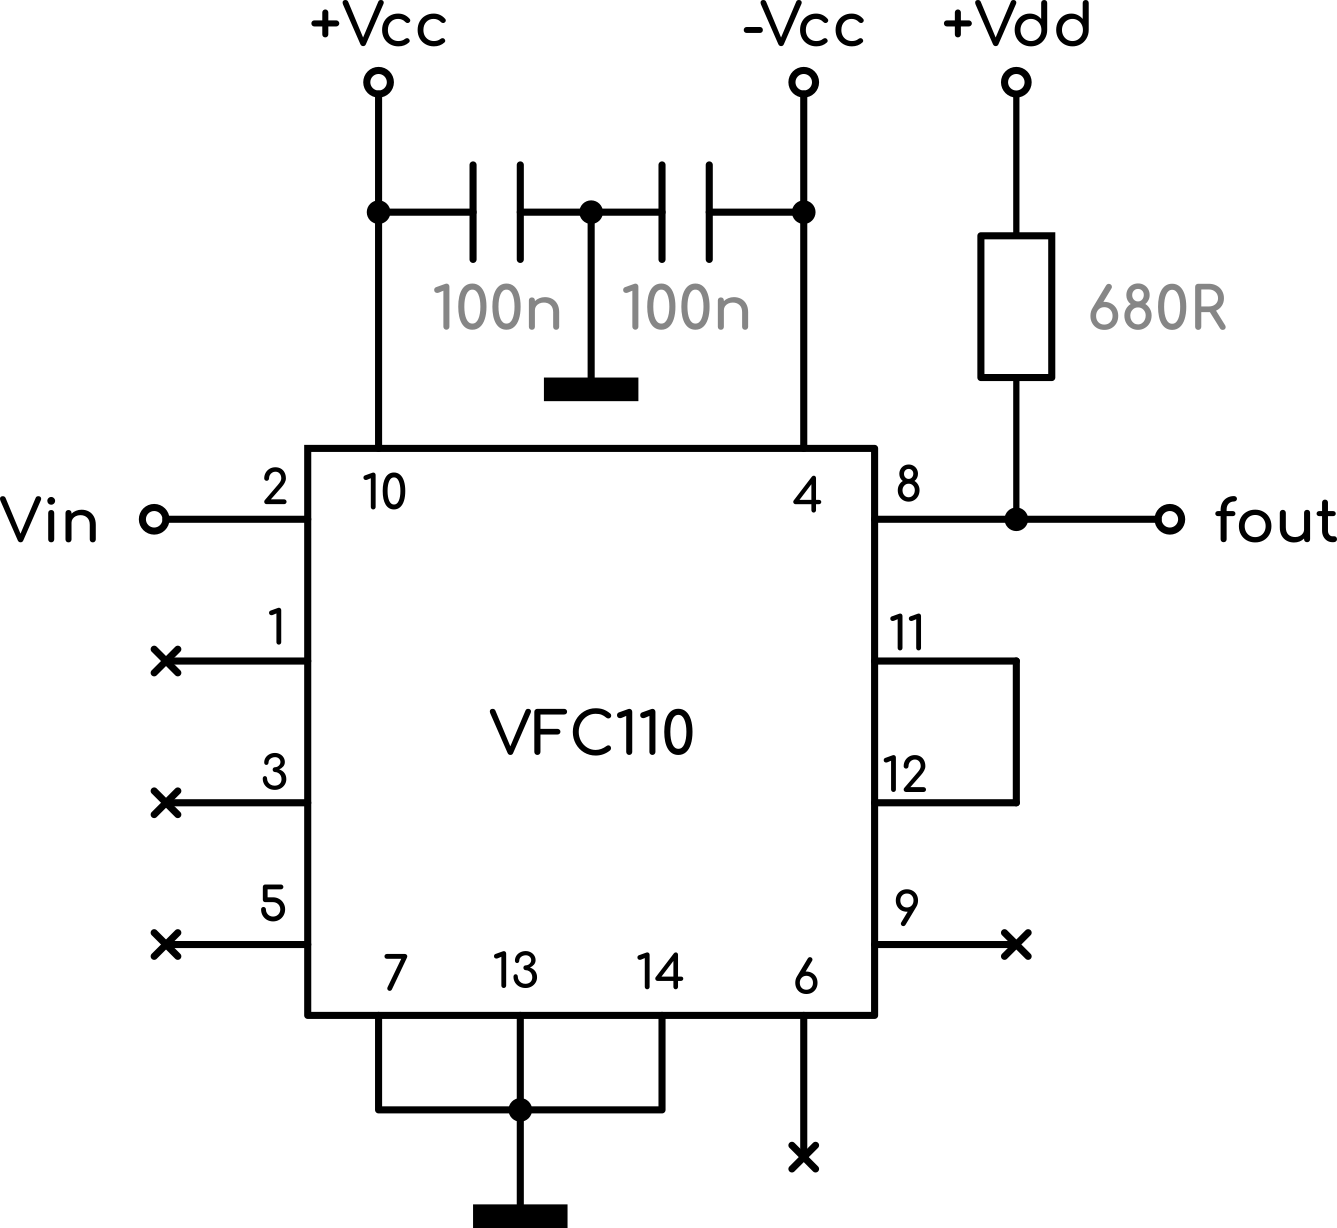
\includegraphics{circuits/VFC_circuit.png}
    \caption{Schema elettrico del circuito utilizzato ($\pm V_{cc}=\pm 12\ V$, $+V_{}=+5\ V$)}
    \label{VFC_circuit}
\end{figure}

Si noti che gli unici componenti aggiunti sono condensatori di filtro e un resistore di
pull-up per l'uscita a collettore aperto.

Si riportano anche le relazioni tra le principali grandezze in gioco:

\begin{equation}\label{duty_cycle}
    I_{in}=I_{ref}\cdot\delta\ [A]
    \qquad
    \rightarrow
    \qquad
    \delta=\frac{I_{in}}{I_{ref}}=\frac{V_{in}}{R_{in}\cdot I_{ref}}
\end{equation}

\begin{equation}\label{fout}
    \frac{V_{in}}{R_{in}}=I_{ref}\cdot f_{out}\cdot T_{OS}\ [A]
    \qquad
    \rightarrow
    \qquad
    f_{out}=\frac{V_{in}}{R_{in}\cdot I_{ref}\cdot T_{OS}}=\frac{\delta}{T_{OS}}\ [Hz]
\end{equation}

%--------------------------------------------------------------------------------------------

\subsection*{Risultati Pratici e Misure}

%--------------------------------------------------------------------------------------------

Si procede quindi alla verifica del corretto funzionamento del circuito. Il setup di
misura utilizzato è il seguente:

\begin{figure}[H]
    \centering
    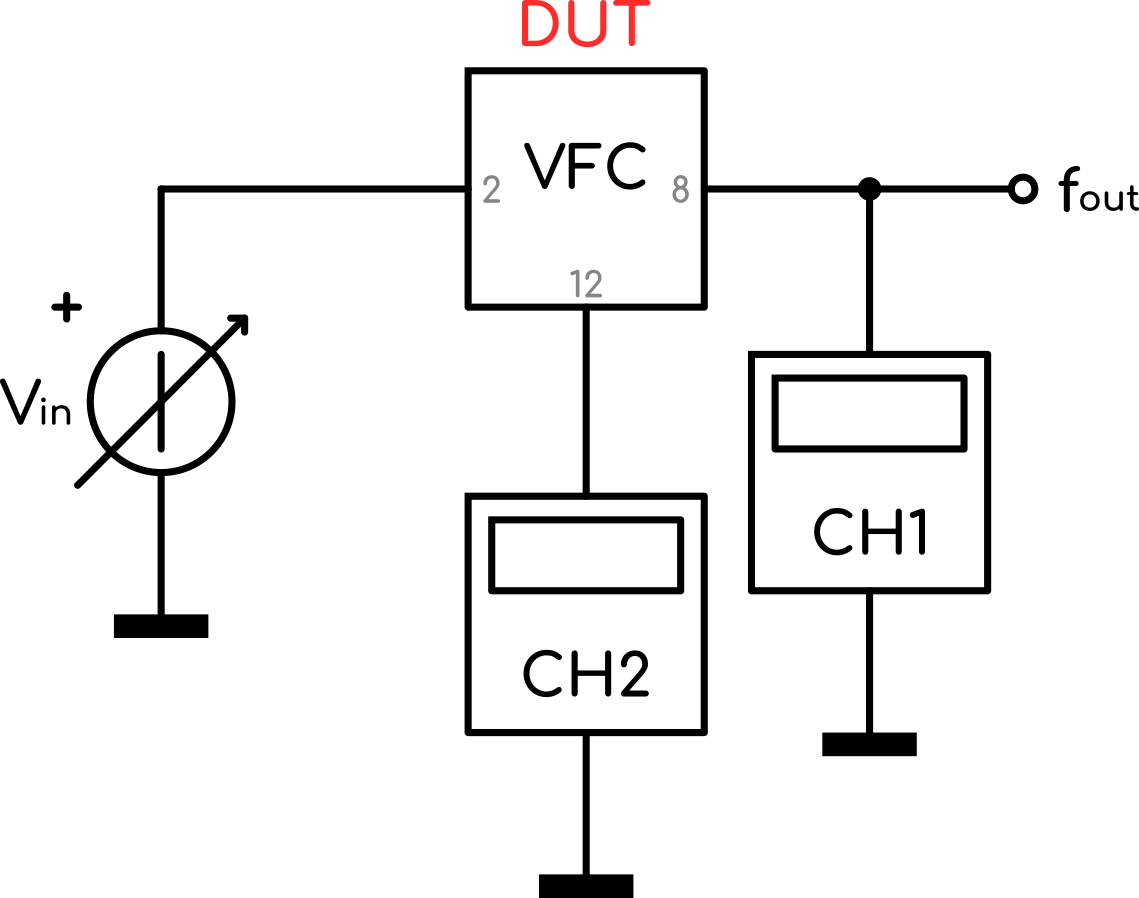
\includegraphics{block_diagrams/mis_VFC.png}
    \caption{Setup di misura del VFC}
    \label{mis_VFC}
\end{figure}

Successivamente si raccolgono in tabella i dati che verranno poi utilizzati per tracciare i
grafici corrispondenti:

\begin{table}[H]
    \centering
    \csvreader[
    tabular = |C||C|L|,
    table head = {\hline \rowcolor{myLightGrey} $V_{in}\ [V]$ & $\delta\ [\%]$ & $f_{out}\ [kHz]$ \\\hline},
    late after line = \\\hline,
    ]{data/misure_vfc.csv}{}{
    \csvcoli & \csvcoliii & \csvcolv
    }
    \caption{Valori misurati del blocco VFC}
    \label{vfc_table}
\end{table}

Possiamo anzitutto verificare che il comportamento dell'integratore corrisponde a quello
descritto nel paragrafo precedente, e si nota che la durata del periodo basso di $f_{out}$
si estende lungo il tratto di rampa crescente come in figura \ref{integrator_behaviour},
ovvero durante il periodo $T_{OS}$, in cui il timer risulta attivo. Possiamo anche
notare che la sua durata non varia in funzione di $V_{in}$ o $f_{out}$, ma rimane invece
pressoché costante a circa $100\ ns$. Questo valore risulta corretto se inserito nella
formula \ref{fout} poichè fornisce una stima accurata dei valori di frequenza misurati.

\begin{figure}[H]
    \centering

    \begin{subfigure}{.5\textwidth}
        \centering
        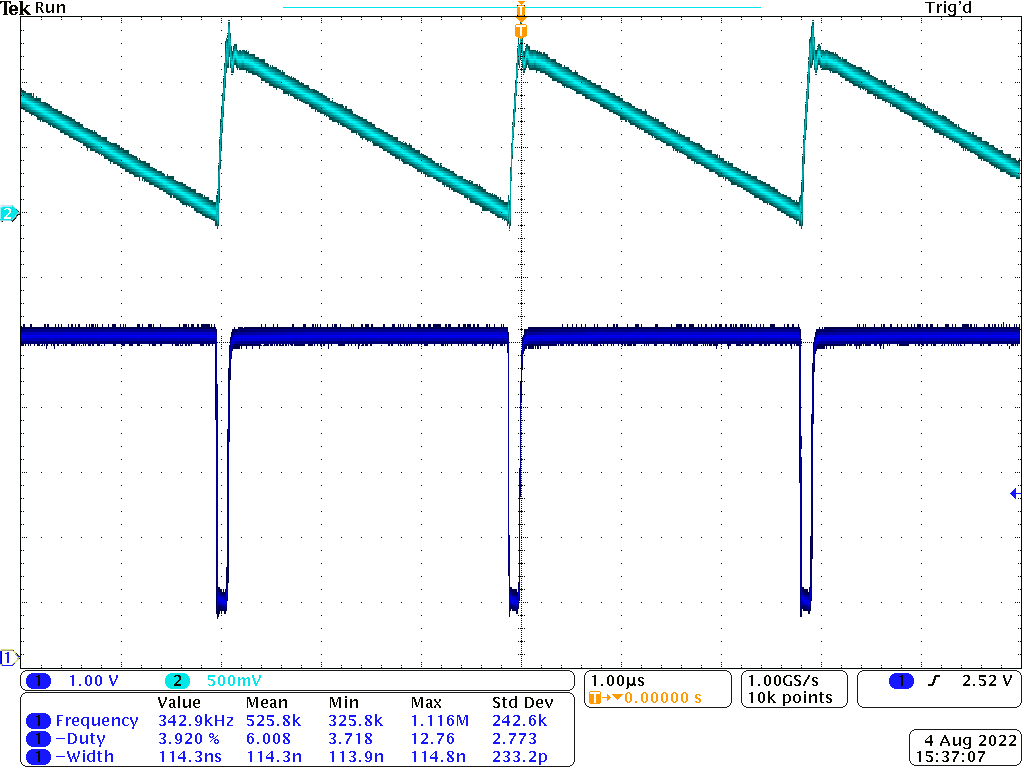
\includegraphics[scale = 0.2]{acquisitions/VFC_1V.png}
        \caption{$V_{in}=1\ V$}
        \label{acq_vfc110_1v}
    \end{subfigure}%
    \begin{subfigure}{.5\textwidth}
        \centering
        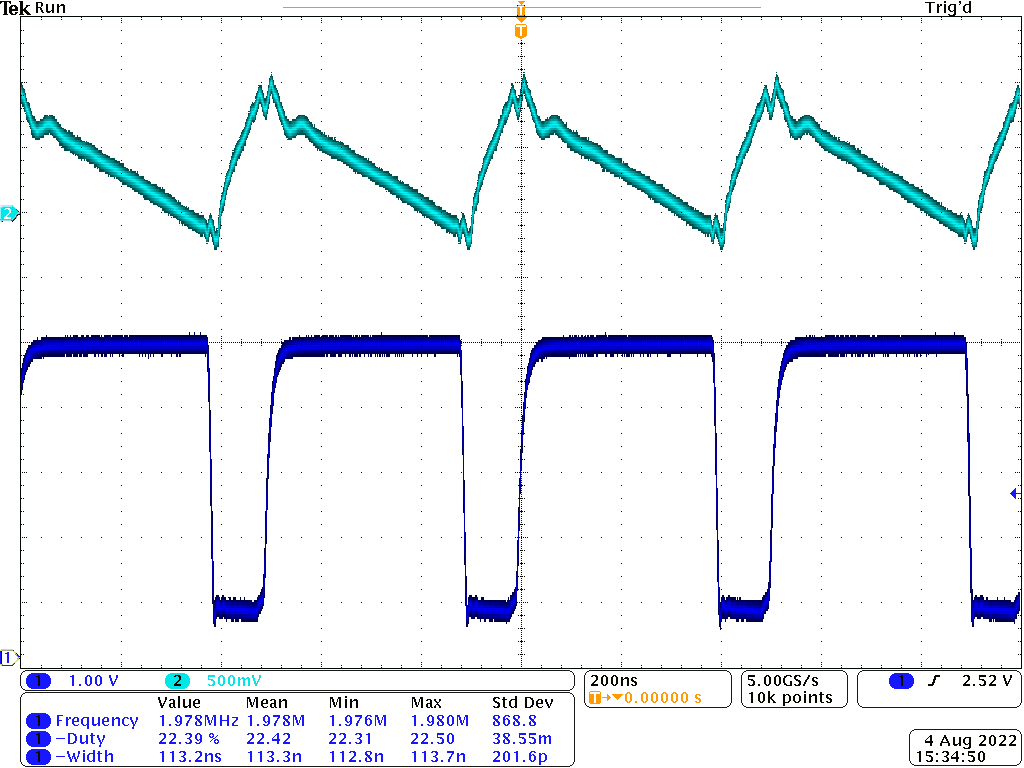
\includegraphics[scale = 0.2]{acquisitions/VFC_5V.png}
        \caption{$V_{in}=5\ V$}
        \label{acq_vfc110_5v}
    \end{subfigure}
    \begin{subfigure}{.5\textwidth}
        \centering
        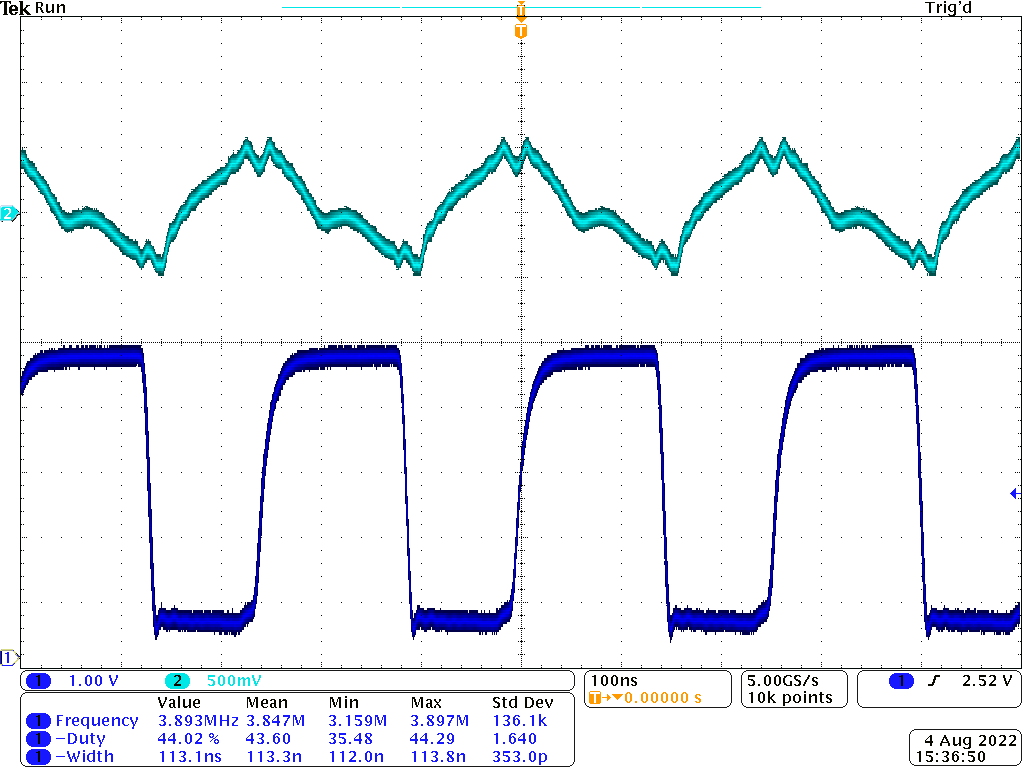
\includegraphics[scale = 0.2]{acquisitions/VFC_10V.png}
        \caption{$V_{in}=10\ V$}
        \label{acq_vfc110_10v}
    \end{subfigure}

    \caption{Acquisizioni dei segnali di interesse per diversi valori di $V_{in}$}
    \label{acq_vfc110}
\end{figure}

\begin{figure}[H]
    \centering

    \begin{subfigure}{.5\textwidth}
        \centering
        \begin{tikzpicture}[scale = 0.85]
            \begin{axis}[
                    title = Duty Cycle,             % title
                    no marks,
                    xmin = 0, xmax = 12,            % limit values
                    ymin = 0, ymax = 50,
                    grid = major,                   % grid
                    grid style = {dashed, gray!30},
                    xlabel = $V_{in}$,              % axis titles and units
                    ylabel = $\delta$,
                    x unit = \si{\V}, y unit = \si{\percent},
                    legend style = {at = {(0.5, -0.25)}, anchor = north},
                    cycle list name = modular,
                ]

                \addplot
                table[x = vin, y = duty atteso, col sep = comma]{./data/misure_vfc.csv};

                \addplot
                table[x = vin, y = duty misurato, col sep = comma]{./data/misure_vfc.csv};

                \legend{Formula \ref{duty_cycle}, Valori misurati}
            \end{axis}
        \end{tikzpicture}
    \end{subfigure}%
    \begin{subfigure}{.5\textwidth}
        \centering
        \begin{tikzpicture}[scale = 0.85]
            \begin{axis}[
                    title = Frequenza,              % title
                    no marks,
                    xmin = 0, xmax = 12,            % limit values
                    ymin = 0, ymax = 5000,
                    grid = major,                   % grid
                    grid style = {dashed, gray!30},
                    xlabel = $V_{in}$,              % axis titles and units
                    ylabel = $f_{out}$,
                    x unit = \si{\V}, y unit = \si{\kHz},
                    legend style = {at = {(0.5, -0.25)}, anchor = north},
                    cycle list name = modular,
                ]

                \addplot
                table[x = vin, y = fout attesa, col sep = comma]{./data/misure_vfc.csv};

                \addplot
                table[x = vin, y = fout misurata, col sep = comma]{./data/misure_vfc.csv};

                \legend{Formula \ref{fout}, Valori misurati}
            \end{axis}
        \end{tikzpicture}
    \end{subfigure}

    \caption{Grafici delle grandezze riportate in tabella \ref{vfc_table}}
    \label{vfc_graphs}
\end{figure}

Si nota che l'andamento del duty cycle si distacca leggermente dalla teoria, pur avendo
comunque un comportamento lineare. Questo è dovuto probabilmente a causa di diverse
non-idealità del componente, come ad esempio le tolleranze dei componenti interni al
VFC110, tuttavia il parametro di maggiore interesse in questo caso è $f_{out}$, che invece
risulta quasi uguale ai valori calcolati, come evidente in figura \ref{vfc_graphs}b.

%--------------------------------------------------------------------------------------------

\chapter{Condizionamento dell'Ingresso}

%--------------------------------------------------------------------------------------------

\section{Convertitore Lineare-Esponenziale}

%--------------------------------------------------------------------------------------------

Vogliamo ora analizzare la sezione di circuto che soddisfa la specifica sulla modalità
$1V/Octave$ dell'ingresso, ovvero il circuito in grado di convertire una tensione
lineare in una esponenziale.

%--------------------------------------------------------------------------------------------

\subsection*{Analisi del Circuito}

%--------------------------------------------------------------------------------------------

Per l'applicazione si sfrutta la caratteristica esponenziale intrinseca del transistor
bipolare:

\begin{displaymath}
    i_e\approx i_c=I_se^{\left(\frac{v_{be}}{V_T}-1\right)}
    \approx I_se^{\left(\frac{v_{be}}{V_T}\right)}
\end{displaymath}

\begin{figure}[ht]
    \centering
    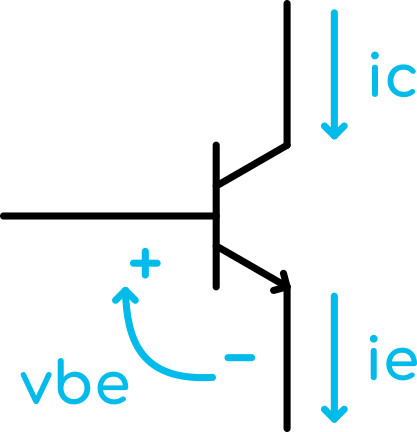
\includegraphics{circuits/single_transistor_circuit.png}
    \caption{BJT}
    \label{bjt}
\end{figure}

dove $V_T$ (o potenziale termico) e $I_s$ (o corrente di saturazione) sono variabili in
funzione della temperatura, ad ogni modo nella nostra analisi considereremo $V_T$ costante
a $26mV$.

Per rimuovere dall'equazione $I_s$ invece, si collegano 2 transistor (idealmente nello
stesso chip, in modo che siano il più possibile simili tra loro e termicamente accoppiati)
in configurazione a coppia differenziale:
\medskip

\begin{figure}[ht]
    \centering
    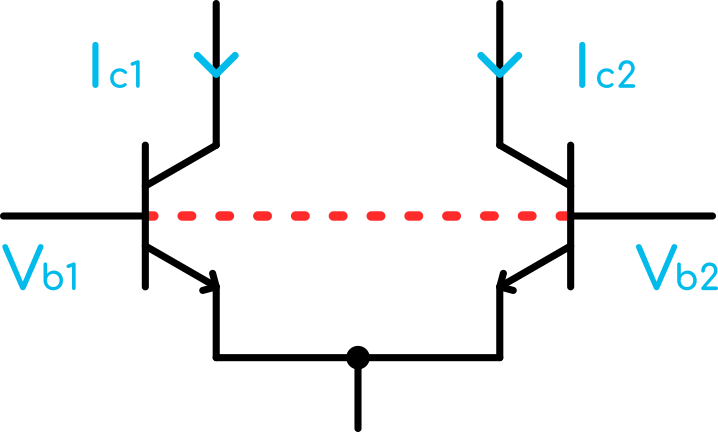
\includegraphics{circuits/differential_pair_circuit.png}
    \caption{Coppia differenziale a BJT}
    \label{differential_pair_circuit}
\end{figure}

per la quale vale la seguente relazione:

\begin{displaymath}
    \frac{i_{c2}}{i_{c1}}=\frac{I_s e^{\left(\frac{v_{be2}}{V_T}\right)}}{I_s e^{\left(\frac{v_{be1}}{V_T}\right)}}
    \qquad
    \rightarrow
    \qquad
    i_{c2}=i_{c1}e^{\left(\frac{v_{be2}-v_{be1}}{V_T}\right)}=i_{c1}e^{\left(\frac{v_{b2}-v_{b1}}{V_T}\right)}
\end{displaymath}

dove risulta evidente che la dipendenza da $I_s$ viene completamente rimossa.

A questo punto, apportiamo alcune modifiche al circuito:

\begin{figure}[ht]
    \centering
    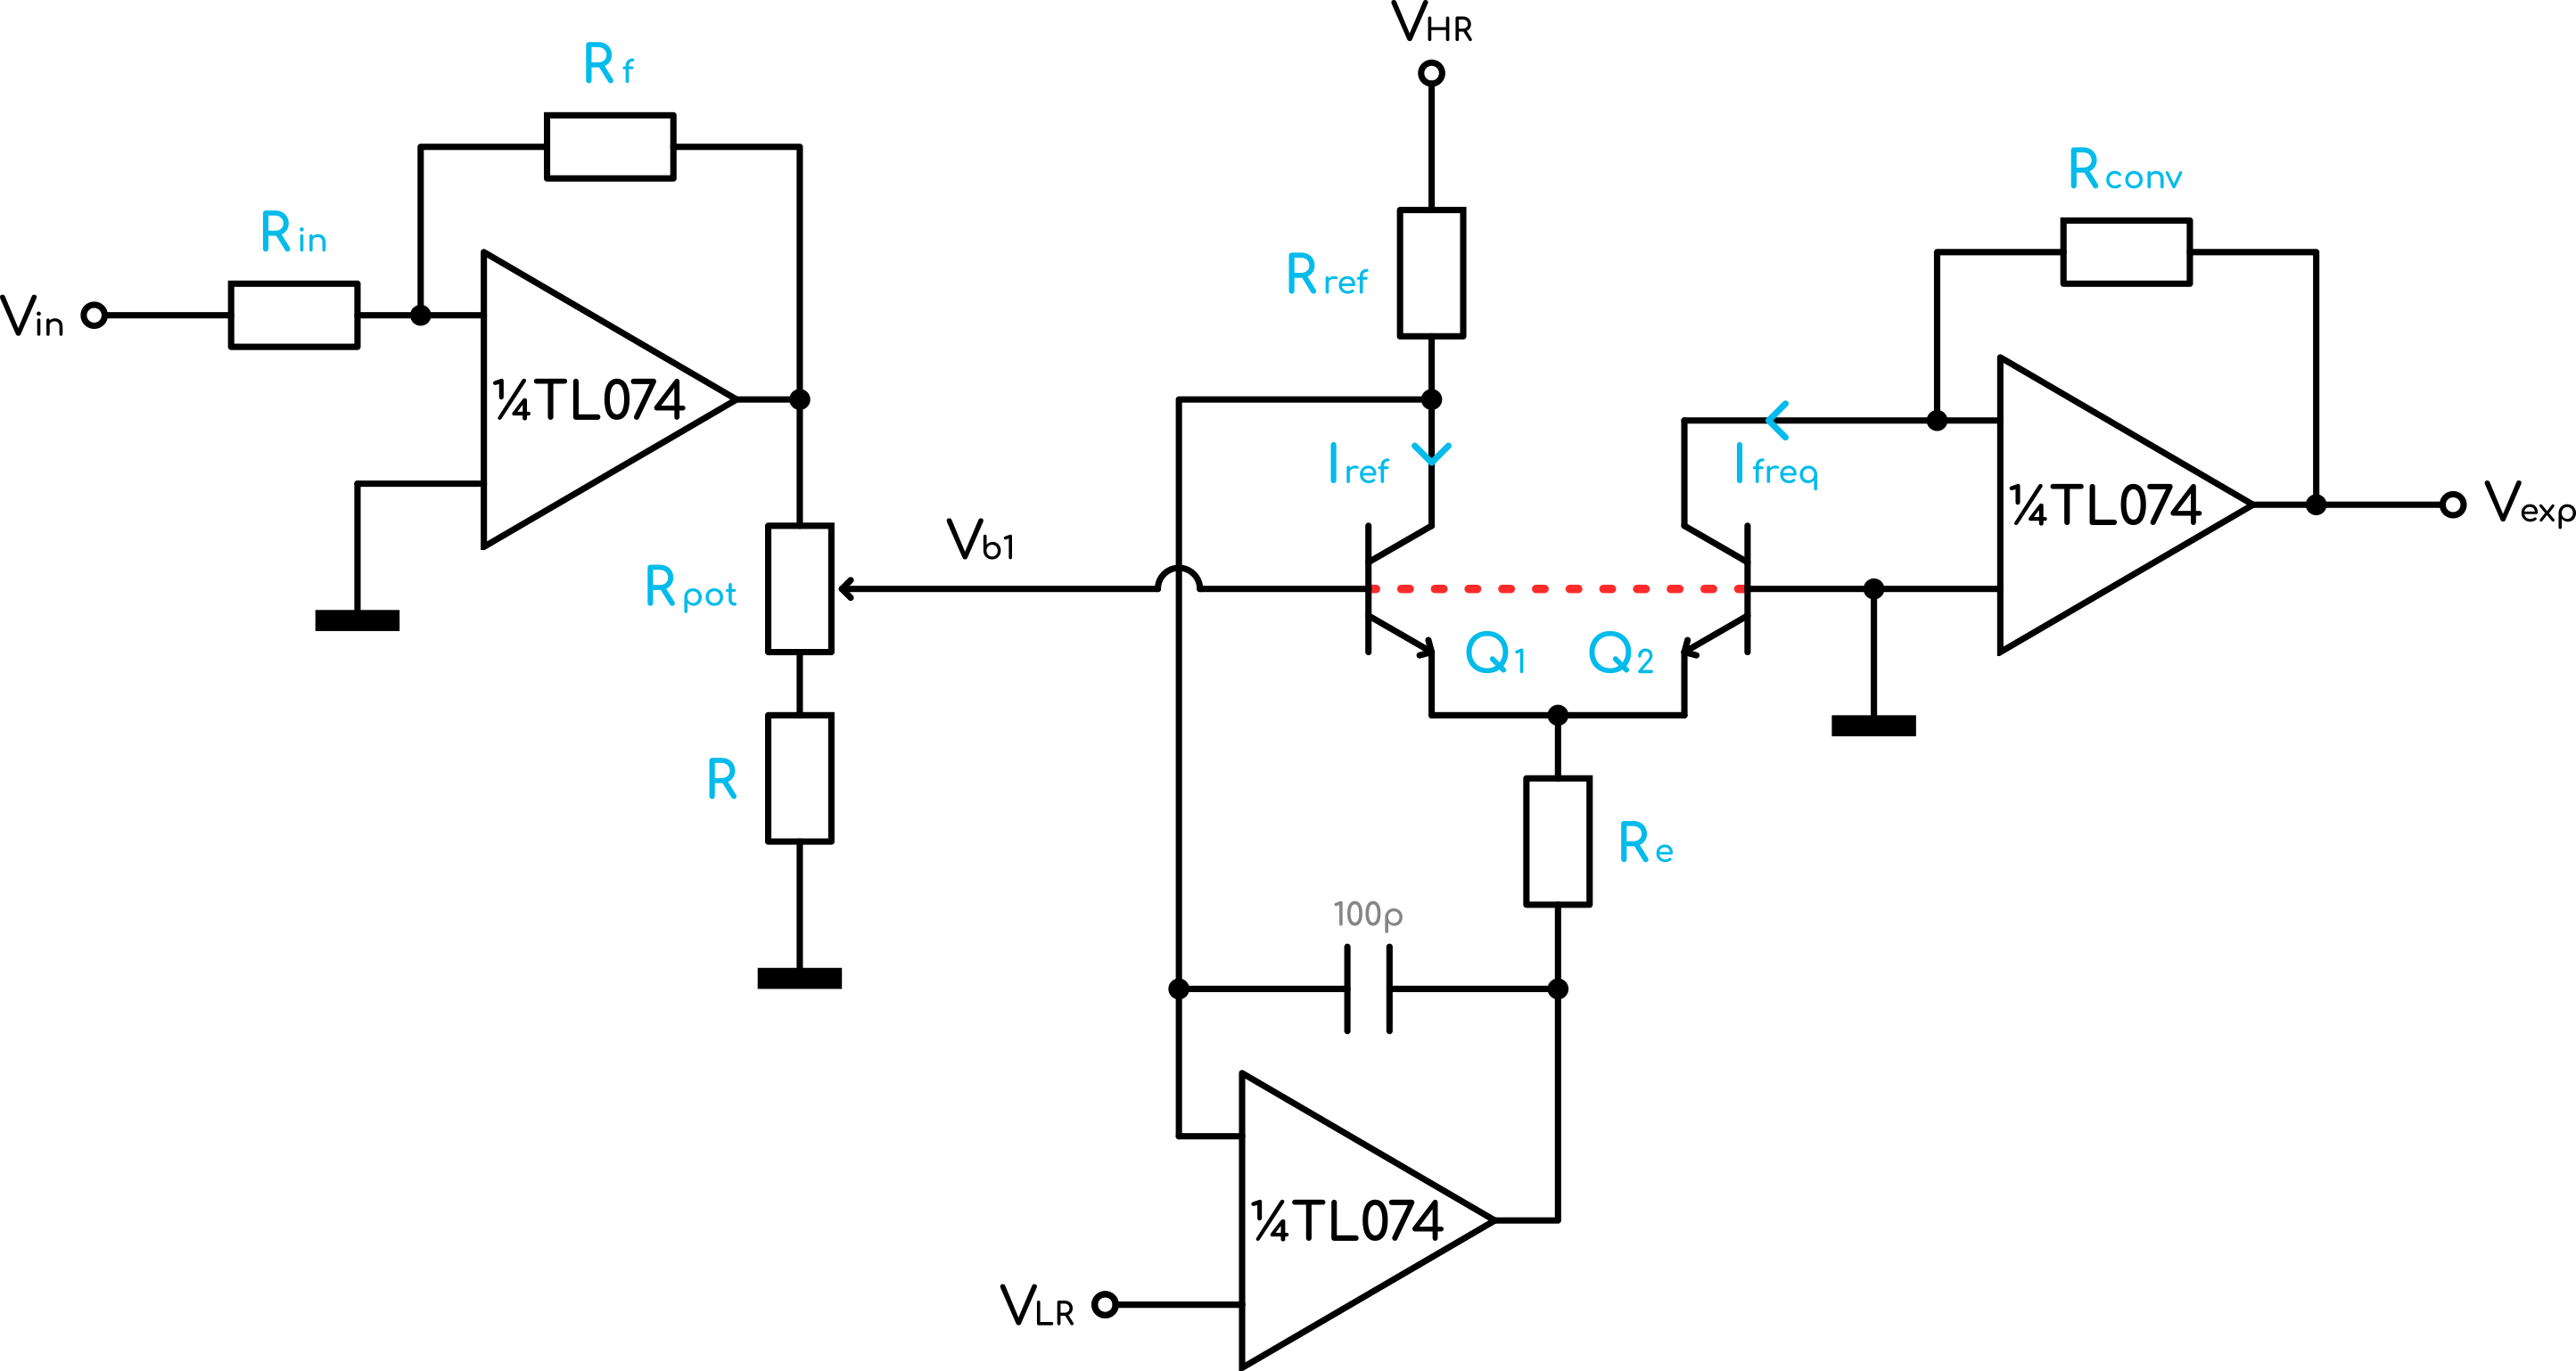
\includegraphics{circuits/exponential_converter_circuit.png}
    \caption{Convertitore tensione lineare - corrente esponenziale}
    \label{exponential_converter_circuit}
\end{figure}

dove l'operazionale di sinistra si occupa di invertire il segno della tensione di ingresso
per avere un valore positivo all'esponente, mentre quello di destra si occupa di mantenere
costante la corrente di riferimento $I_{ref}$.

Valgono quindi:

\begin{displaymath}
    i_{freq}=I_{ref}e^{-\frac{v_{b1}}{V_T}}
\end{displaymath}

\begin{displaymath}
    I_{ref}=\frac{V_{HR}-V_{LR}}{R_{ref}}
\end{displaymath}

Ora per completare il tutto basta aggiungere un convertitore corrente-tensione al collettore
di $Q_2$, legando cosi $V_{in}$ a $V_{out}$ con la seguente relazione:

\begin{displaymath}
    V_{out}=R_f\cdot i_{freq}=
    R_f\cdot I_{ref}e^{-\frac{v_{b1}}{V_T}}=
    R_f\cdot \frac{V_{HR}-V_{LR}}{R_{ref}}e^{-\frac{s\cdot V_{in}}{V_T}}
\end{displaymath}

% circuito completo con IVC figura 4

%--------------------------------------------------------------------------------------------

\subsection*{Dimensionamento e Scelta dei Componenti}

%--------------------------------------------------------------------------------------------

Passiamo quindi al dimensionamento dei componenti, in modo da imporre al circuito il
comportamento voluto.

Come prima cosa calcoliamo il valore del guadagno $s$ dell'amplificatore invertente.
Si vuole:

\begin{displaymath}
    i_{freq}=I_{ref}e^{-\frac{s\cdot V_{in}}{V_T}}
    \qquad
    \rightarrow
    \qquad
    2i_{freq}=I_{ref}e^{-\frac{s\cdot[V_{in}+\Delta V_{in}]}{V_T}}
\end{displaymath}

qundi un raddoppio della corrente $i_{freq}$ per ogni variazione $\Delta V_{in}=1V$.
Allora possiamo riscrivere le due relazioni nel seguente modo:

\begin{displaymath}
    2=e^{-\frac{s\cdot\Delta V_{in}}{V_T}}
    \qquad
    \rightarrow
    \qquad
    ln(2)=-\frac{s\cdot\Delta V_{in}}{V_T}
    \qquad
    \rightarrow
    \qquad
    -s=\frac{V_T\cdot ln(2)}{\Delta V_{in}}
\end{displaymath}

e sostituendo i valori otteniamo:

\begin{displaymath}
    -s=\frac{26mV\cdot 0.6931}{1V}\approx-0.018\approx-\frac{1}{55.5}
\end{displaymath}

valore che può essere diviso nel seguente modo:

\begin{displaymath}
    s=\bar{s}\cdot\hat{s}=\frac{2k\Omega}{100k\Omega}\cdot\frac{440\Omega}{490\Omega}
    \approx 0.018
\end{displaymath}

quindi:

% circuito amplificatore completo figura 5

\begin{itemize}
    \item $R_f = 2k\Omega$;
    \item $R_{in} = 100k\Omega$;
    \item $R_{pot} = 100\Omega$;
    \item $R = 390\Omega$;
\end{itemize}

impostiamo i valori di $V_{HR}=+12V$ e $V_{LR}=0V$.

%--------------------------------------------------------------------------------------------

\subsection*{Risultati Pratici e Misure}

%--------------------------------------------------------------------------------------------

testo

%--------------------------------------------------------------------------------------------

\section{Somma di più Ingressi}

%--------------------------------------------------------------------------------------------

testo

%--------------------------------------------------------------------------------------------

\section{Clipper}

%--------------------------------------------------------------------------------------------

testo

%--------------------------------------------------------------------------------------------

\subsection*{Risultati Pratici e Misure}

%--------------------------------------------------------------------------------------------

\include{chapters/ch04-selezione_modalità.tex}
\chapter{Generazione dei Segnali Secondari}

TODO


\section{Onda Quadra}

TODO


\section{Dente di Sega}

TODO


\section{Sinusoide}

TODO


\section{Impulso}

TODO
\chapter{Stadi di Uscita}

\lipsum[2-4]
\chapter{Protezione del Circuito}

\lipsum[2-4]
\chapter{Composizione delle Schede}

\lipsum[2-4]
\unchapter{Considerazioni Finali e Conclusioni}

TODO

% aggiungere appendice con schemi elettrici

% bibliografia
\printbibliography
\addcontentsline{toc}{chapter}{Bibliografia}

% fine del documento
\end{document}